\documentclass[12pt]{article}
\usepackage[utf8]{inputenc}
\usepackage{graphicx}
\usepackage[spanish,es-tabla]{babel}
\usepackage{amsmath}
\usepackage[a4paper,margin=1in]{geometry}
\usepackage{subcaption}
\captionsetup[subfigure]{listof=true}
\usepackage{amssymb}
\usepackage[hidelinks]{hyperref}
\usepackage{mathtools}
\usepackage[table,xcdraw]{xcolor}
\usepackage[style=ieee, backend=biber]{biblatex}
\usepackage{enumitem}
\usepackage{array}
\usepackage{longtable}
\usepackage{csquotes}
\usepackage{circuitikz}
\usepackage{hyperref}
\usepackage{url}    
\graphicspath{{Figuras/}}           
\usepackage{float}
\usepackage{setspace}
\onehalfspacing

\addbibresource{bibliografía.bib}   
\hypersetup{
    colorlinks=true,
    linkcolor=blue,    
    citecolor=blue,
    urlcolor=blue,
    filecolor=blue
}

\begin{document}       
\renewcommand{\figureautorefname}{Fig.}
\renewcommand{\tableautorefname}{Tab.}
\renewcommand{\equationautorefname}{Ec.}

\begin{titlepage}
\thispagestyle{empty}
\begin{tikzpicture}[remember picture,overlay]
    \node[opacity=0.2,anchor=center] at (current page.center) 
        {
\includegraphics[width=0.9\paperwidth]{decoracion_a.png}};
\end{tikzpicture}
\begin{center}
    
\includegraphics[width=15cm]{unc_fcefyn_logo.png} \\ [0.5cm]
    \LARGE Universidad Nacional de Córdoba \\ [0.5cm] 
    \large Facultad de Ciencias Exactas, Físicas y Naturales \\ 
    \vspace{40pt}
    \large Sistemas de Radiocomunicación \\ [0.2cm]
    \large Trabajo Práctico N°3 \\
    \vspace{60pt}
    \LARGE Fibra Óptica \\
    \vspace{60pt}
    \begin{table}[!h]
        \centering
        \begin{tabular}{ll}
            \multicolumn{1}{c}{Nombre} & \multicolumn{1}{c}{DNI} \\
            Arteaga Barrera, Cristian Eduardo & 95.159.096 \\
            Baccino, Luca & 45.328.380 \\
            Mendes Rosa, Agustín             & 44.517.201 \\
            Monja, Ernesto Joaquín           & 43.873.728 \\

        \end{tabular}
    \end{table}
    \vspace{20pt}
    \begin{table}[!h]
        \centering
        \begin{tabular}{ll}
            \multicolumn{1}{c}{Docentes} & Esp. Ing. Liendo, Carlos Guillermo \\
                                         & Ing. Dadam, Federico Tomás \\
        \end{tabular}
    \end{table}
    \vfill
        {\small Córdoba, República Argentina\\
                Año 2026}
\end{center}
\end{titlepage}
\newpage


\tableofcontents
\newpage
\listoffigures
\newpage

\section{Introducción}

El presente informe tiene como objetivo principal comprender, analizar y comprobar empíricamente los principios físicos y electrónicos que rigen el funcionamiento de los enlaces ópticos.

Para llevar a cabo las experiencias se empleó el kit educativo de fibra óptica EFO1101, abordando el estudio desde dos enfoques principales. En primera instancia, se evaluó la transmisión de señales en modo analógico, contrastando la propagación no guiada en el espacio libre frente a la propagación guiada mediante reflexión total interna en cables de fibra óptica. 

En segunda instancia, se analizó la transmisión en modo digital. A través de la instrumentación con osciloscopio, se caracterizaron los niveles de tensión del circuito, la importancia del umbral de decisión frente a la atenuación del medio, y las limitaciones físicas del sistema al operar en las frecuencias extremas de su ancho de banda. De esta manera, se busca establecer una correlación directa entre la teoría de componentes ópticos, la propagación de ondas electromagnéticas y el comportamiento real de los circuitos acondicionadores de señal.


\section{Marco Teórico}

\subsection{Sistemas de Comunicaciones Ópticas}
Un sistema de comunicación óptica convierte una señal eléctrica de información en una onda electromagnética en el espectro óptico, transmite la luz a través de un canal y la reconvierte en una señal eléctrica en el receptor (ver \autoref{fig:diagrama1}). El canal de transmisión puede ser el espacio libre (propagación no guiada) o un medio confinado como la fibra óptica (propagación guiada).

\begin{figure}[H]
    \centering
    \fbox{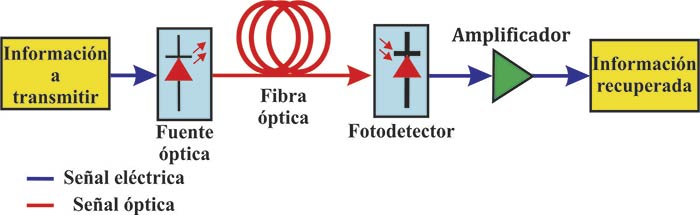
\includegraphics[width=0.6\linewidth]{diagrama1.png}}
    \caption{Diagrama elemental de un sistema de comunicación óptico.}
    \label{fig:diagrama1}
\end{figure}

\subsection{Propagación por Espacio Libre y en Fibra Óptica}

\subsubsection{Transmisión en Espacio Libre}
En espacio libre, la radiación emitida por la fuente viaja y obedece las leyes de la óptica geométrica, como la ley de reflexión especular, donde el ángulo de incidencia es igual al ángulo de reflexión respecto a la normal en el mismo medio. Esto permite la manipulación y redireccionamiento del haz de luz mediante elementos reflectantes externos (como es el caso de espejos).

\subsubsection{Estructura de la Fibra Óptica y Reflexión Total Interna}
La fibra óptica es un conductor de luz con muy baja atenuación (en relación a los cables coaxiales), tal que se pueden lograr comunicaciones de miles de kilómetros. Consta de un núcleo cilíndrico construido de dióxido de silicio ($SiO_2$) con índice de refracción $n_1$, rodeado por un revestimiento con índice de refracción $n_2$, donde se cumple que $n_1 > n_2$ \cite{pres1}.

El confinamiento y guiado de la luz dentro del núcleo se basa en el fenómeno de la Reflexión Total Interna (RTI). La refracción en la interfaz núcleo-revestimiento se rige por la Ley de Snell (donde sí existe una refracción por cambio de medios):

\begin{equation}
n_1 \sin(\theta_i) = n_2 \sin(\theta_t)
\end{equation}

donde $\theta_i$ es el ángulo de incidencia y $\theta_t$ es el ángulo de refracción, medidos respecto a la normal de la interfaz \cite{pres1}. 

El ángulo crítico ($\theta_c$) es el ángulo mínimo de incidencia a partir del cual no existe rayo refractado hacia el revestimiento ($\theta_t = 90^\circ$), reflejándose toda la energía dentro del núcleo \cite{pres1}:

\begin{equation}
\theta_c = \arcsin\left(\frac{n_2}{n_1}\right)
\end{equation}

\subsubsection{Cono de Aceptación y Apertura Numérica}

Para que la luz ingresada por el extremo de la fibra cumpla la condición de RTI, debe ingresar dentro de un límite angular denominado cono de aceptación \autoref{fig:Cono}. La capacidad de captación de luz de la fibra se define mediante la Apertura Numérica (AN), es decir, el nivel de aceptancia de la FO para captar la energía entregada por la fuente óptica:

\begin{equation}
\text{AN} = \sin(\alpha_{\text{máx}}) \approx n_1 \cdot \sin(\theta_c) = \sqrt{n_1^2 - n_2^2} 
\end{equation}

donde $\alpha_{\text{máx}}$ representa el ángulo máximo de aceptación en el aire ($n_0 \approx 1$) \cite{pres1} \cite{pres2}.

\begin{figure}[H]
    \centering
    \fbox{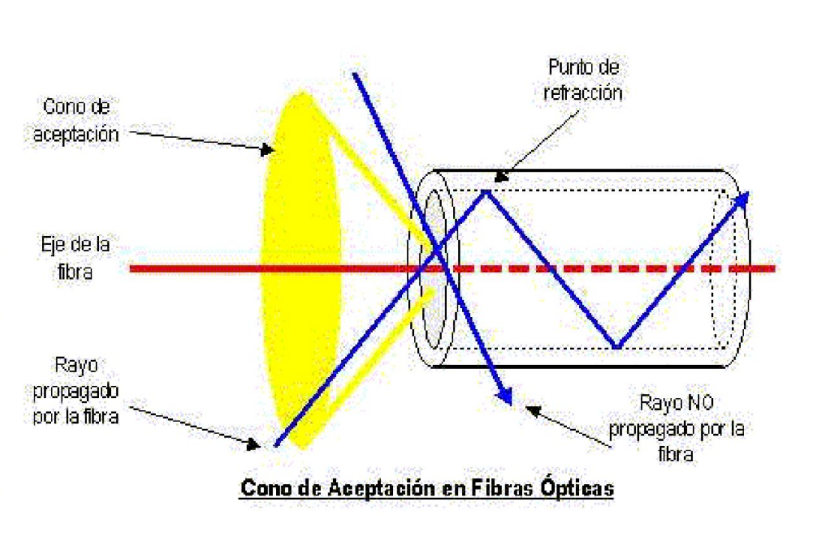
\includegraphics[width=0.5\linewidth]{Cono.png}}
    \caption{Cono de aceptación.}
    \label{fig:Cono}
\end{figure}


\subsection{Componentes utilizados en FO}

\subsubsection{Emisores de Luz}
Los transmisores utilizan Diodos Emisores de Luz (LEDs) que operan tanto en el espectro visible como en el infrarrojo \cite{pres3}.

\subsubsection{Detectores de Luz}
El receptor emplea fotodiodos para convertir la potencia óptica incidente en una corriente eléctrica proporcional \cite{pres3}. Sus principales parámetros son:

\begin{itemize}
    \item \textbf{Sensibilidad Mínima [dBm]}: Mínima potencia de entrada necesaria para garantizar la correcta detección de bits o la calidad de la señal.
    
    \item \textbf{Potencia Máxima Admisible [dBm]}: Nivel de potencia límite que la interfaz del receptor puede soportar sin saturarse.
    
    \item \textbf{Responsividad [A/W]}: Relación entre la corriente de salida y la potencia óptica de entrada. Mide la eficiencia de conversión.
    
    \item \textbf{Reflectancia:} Cuánto devuelve el sensor de la luz incidente.
\end{itemize}


\subsection{Clasificación y Características de las Fibras Ópticas}

Las fibras ópticas se clasifican principalmente según el número de modos (trayectorias electromagnéticas) que permiten propagar en su interior, según la distribución del índice de refracción dentro del núcleo.

\subsubsection{Clasificación según los Modos de Propagación}

\begin{itemize}
    \item \textbf{Fibra Monomodo (SMF - \textit{Single-Mode Fiber}):}
    Posee un núcleo muy estrecho, típicamente de $8\text{ a } 10\,\mu\text{m}$ de diámetro. Debido a estas dimensiones tan reducidas respecto a la longitud de onda de trabajo ($\lambda$), solo se permite la propagación del modo fundamental \cite{pres1}.

    \item \textbf{Fibra Multimodo (MMF - \textit{Multi-Mode Fiber}):}
    Posee un núcleo sustancialmente mayor, típicamente de $50\,\mu\text{m}$ de diámetro. Permite que múltiples modos de luz viajen simultáneamente a través de diferentes ángulos de transmisión \cite{pres1}.
    
    Sufre de dispersión modal, ya que los diferentes modos recorren distancias distintas y llegan en tiempos diferentes al fotodetector, provocando ensanchamiento de los pulsos digitales y limitando la distancia y la velocidad máxima de transmisión \cite{wiki}.
\end{itemize}

\begin{figure}[H]
    \centering
    \fbox{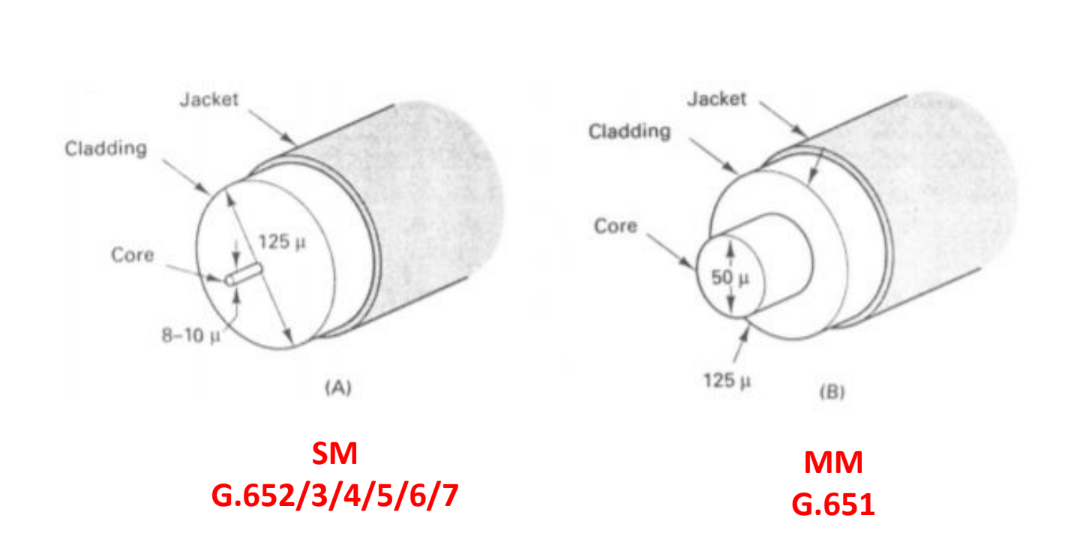
\includegraphics[width=0.7\linewidth]{Modos.png}}
    \caption{Dimensiones del cable según los modos.}
    \label{fig:Modos}
\end{figure}


\subsection{Atenuación}
La atenuación cuantifica la pérdida de potencia que sufre la señal óptica al propagarse por el medio de transmisión:

\begin{equation}
\alpha \, [\text{dB}] = 10 \log_{10}\left(\frac{P_{\text{entrada}}}{P_{\text{salida}}}\right)
\end{equation}

La fibra óptica más moderna tiene una atenuación de $0.15 \, [dB/km]$, es decir, cada $20 \, [km]$ la señal se reduce a la mitad de potencia \cite{pres2}.

Debido a las pérdidas por longitud, un cable óptico largo presenta mayor atenuación que uno corto. Para mitigar esto en el receptor digital, se debe incrementar la potencia del emisor o ajustar el nivel del umbral digital, ya que si la señal que llega al receptor es muy débil, el receptor no detecta correctamente los bits y la tasa de error aumenta.

Las curvas de la \autoref{fig:Atenuacion} muestran la variación del nivel de atenuación según incrementa la longitud de onda, para distintos tipos de fibra \cite{pres2}.

\begin{figure}[H]
    \centering
    \fbox{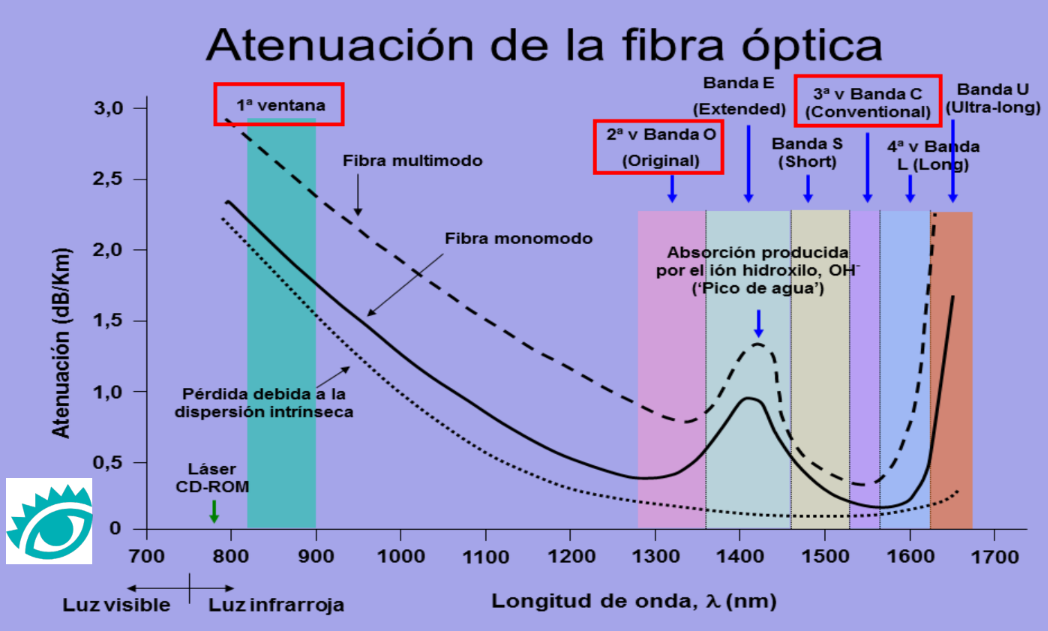
\includegraphics[width=0.75\linewidth]{Atenuacion.png}}
    \caption{Curvas de Atenuación según Longitud de Onda.}
    \label{fig:Atenuacion}
\end{figure}

El ``Pico de Agua'' que logra verse es un aumento en la atenuación de la señal, causado cuando los iones hidróxido ($OH^-$) atrapados en el vidrio absorben longitudes de onda específicas al reaccionar con la humedad. Actualmente se fabrican fibras que casi no tienen pico de agua, llamadas fibras ZWPF (\textit{Zero Water Peak Fiber}) o fibras LWP (\textit{Low Water Peak}) \cite{wiki2}.


\subsection{Modulación Óptica: Modo Analógico y Digital}

En los sistemas de comunicaciones por fibra óptica, la información eléctrica puede modular a la fuente de luz principalmente de dos maneras, dependiendo de la naturaleza de la señal a transmitir:

\subsubsection*{Modulación Analógica}
En este modo, la intensidad de la luz emitida por el LED es directamente proporcional a la tensión de la señal eléctrica de entrada. Para evitar recortes en la señal (ya que la luz no puede tener valores negativos), se suma un nivel de tensión de continua (sesgo o \textit{DC bias}) a la señal alterna de información. De esta forma, el fotodetector en el receptor genera una fotocorriente que reproduce fielmente las variaciones continuas de amplitud de la onda original.

\subsubsection*{Modulación Digital}
En las comunicaciones digitales, la señal óptica no varía de forma continua, sino que se emplea un esquema de modulación de amplitud conmutada. En el transmisor, la fuente de luz conmuta entre dos estados lógicos: un nivel de alta intensidad lumínica para representar un bit ``1'', y un nivel de baja intensidad (o apagado) para representar un bit ``0''.

En el receptor, la corriente generada por el fotodiodo es convertida a un nivel de tensión, el cual ingresa a un circuito comparador. Este circuito evalúa la señal recibida frente a un nivel de referencia preestablecido conocido como umbral de decisión (threshold). 

\begin{itemize}
    \item Si el nivel de la señal detectada supera el umbral, el sistema reconstruye un 1 lógico.
    \item Si el nivel de la señal se encuentra por debajo del umbral, el sistema asume que se recibió un 0 lógico.
\end{itemize}

El ajuste correcto de este umbral es crítico: si la señal sufre mucha atenuación en el trayecto y la potencia recibida no logra superar el nivel de umbral configurado, el receptor no podrá regenerar la señal, interrumpiendo la comunicación.
\newpage

\section{Consideraciones y Medidas de Seguridad para la Manipulación de Fibra Óptica}

\subsection{Advertencia General y Riesgos Asociados}
La manipulación de elementos relacionados con la fibra óptica presenta riesgos que dependen tanto de la naturaleza de la radiación lumínica como de las propiedades mecánicas del núcleo de vidrio. Para evitar accidentes personales y daños en los componentes del kit educativo, es obligatorio cumplir con las normas de seguridad durante el desarrollo de la práctica.

\subsection{Seguridad Óptica y Protección Ocular}
Las fuentes de luz utilizadas concentran alta densidad de potencia óptica en áreas reducidas. Dado que gran parte de las transmisiones operan en el espectro infrarrojo no visible, el ojo humano no activa el reflejo de parpadeo de forma natural.

\begin{itemize}
    \item \textbf{Prohibición de visión directa:} En ningún momento se debe ver directamente el extremo de una fibra óptica, conector o puerto emisor activo, ni utilizar instrumentos ópticos de aumento sin la debida verificación previa.
    
    \item \textbf{Direccionamiento del haz:} Queda estrictamente prohibido direccionar o apuntar el extremo de una fibra óptica o emisor hacia la cara o los ojos de otra persona.
    
    \item \textbf{Verificación de presencia de luz:} Para comprobar el paso de la señal óptica, se deben utilizar instrumentos auxiliares (como medidores de potencia óptica o fotodetectores) o reflejar el haz sobre superficies difusas a distancia segura, evitando el contacto ocular directo.
\end{itemize}

\subsection{Manipulación Mecánica y Peligro de Astillado}
Debido a que las fibras ópticas están constituidas por hilos de dióxido de silicio ($\text{SiO}_2$) cubiertos por capas protectoras, el corte o fractura inadecuada de estos hilos genera esquirlas de vidrio extremadamente transparentes, pequeñas y afiladas.

\begin{itemize}
    \item \textbf{Radio mínimo de curvatura:} Se deben evitar en todo momento curvas muy pronunciadas o estrangulamientos. Exceder el límite de curvatura puede quebrar o astillar la fibra en su interior, provocando pérdidas por radiación y el riesgo de cortes.
    
    \item \textbf{Prevención de heridas punzantes:} Las esquirlas de fibra pueden penetrar fácilmente en la piel o los ojos. No se deben tocar las puntas desnudas de la fibra ni recoger restos de vidrio con las manos sin protección.
    
    \item \textbf{Disposición de residuos:} Todos los fragmentos sobrantes de fibra cortada deben recogerse inmediatamente y depositarse en contenedores destinados a residuos de vidrio, evitando dejarlos sobre las mesadas de trabajo.
\end{itemize}

\subsection{Higiene, Limpieza y Manejo de Químicos}
Para mantener las terminales de los conectores libres de impurezas sin comprometer la seguridad del operador:

\begin{itemize}
    \item \textbf{Manipulación de Alcohol Isopropílico:} Debe emplearse alcohol isopropílico para la limpieza de conectores o fibras, lejos de fuentes de calor, chispas o arcos eléctricos, evitando el contacto prolongado con la piel y los ojos.
    
    \item \textbf{Higiene personal:} Al finalizar las actividades de laboratorio, o antes de frotarse los ojos, manipular lentes de contacto o ingerir alimentos, es indispensable lavarse bien las manos con abundante agua fría para retirar cualquier partícula adherida a la piel.
\end{itemize}
\newpage

\section{Parte 1: Transmisión en Modo Analógico y Digital}

\subsection{Práctico A: Modo Analógico}

\subsubsection{Materiales Necesarios}
\begin{itemize}
    \item Fuente de alimentación externa (\autoref{fig:alimentacion}).
    \item Cables banana-cocodrilo (\autoref{fig:coco}).
    \item Módulo Transmisor y Módulo Receptor del Kit (\autoref{fig:kit}).
    \item Dispositivo reproductor de audio con salida Jack $3.5\,\text{mm}$.
    \item Cable de audio mono $3.5\,\text{mm}$ a $3.5\,\text{mm}$ (\autoref{fig:jack}).
    \item Espejo de prueba (\autoref{fig:kit}).
    \item Cable óptico corto y cable óptico largo (\autoref{fig:kit}).
\end{itemize}

Las imágenes a continuación muestran las referencias a los elementos de control de operación del Receptor y Transmisor \cite{datasheet}.

\begin{figure}[H]
  \centering
  \begin{subfigure}{0.4\linewidth}
    \fbox{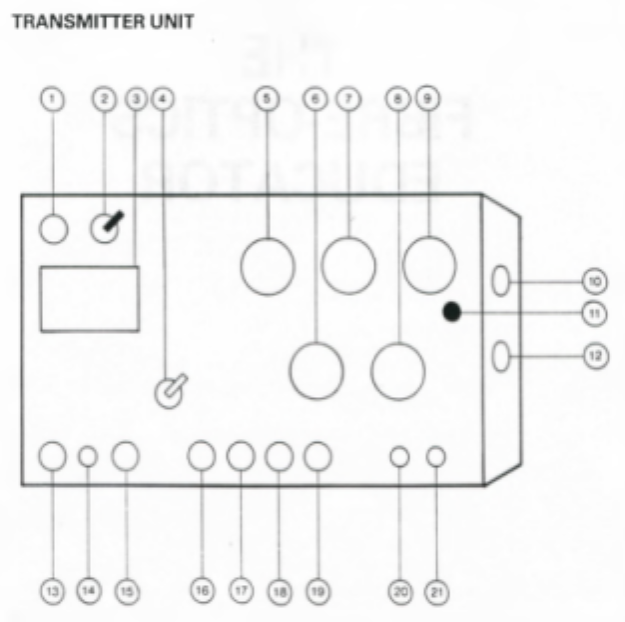
\includegraphics[width=\linewidth]{Transmisor.png}}
    \caption{Transmisor}
    \label{fig:transmisor}
  \end{subfigure}
  \hfill
  \begin{subfigure}{0.45\linewidth}      
    \fbox{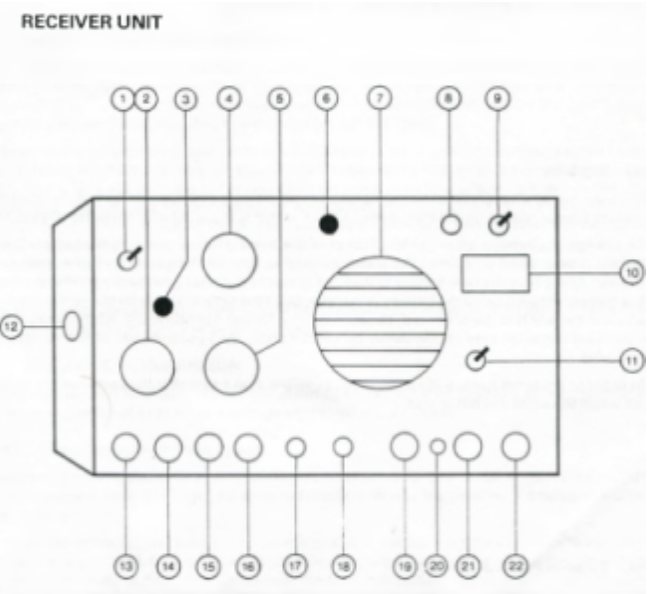
\includegraphics[width=\linewidth]{Receptor.png}}
    \caption{Receptor}
    \label{fig:receptor}
  \end{subfigure}
  \caption{Referencias de Elementos de Control.}
  \label{fig:referencias}
\end{figure}



\subsubsection{Práctico A.1: Transmisión de Señal de Audio por Espacio Libre}

\subsubsection*{Consignas y Procedimiento}
\begin{enumerate}
    \item Colocar el interruptor 11 del receptor en OFF (altavoz de baja impedancia).
    \item Colocar el interruptor 1 del receptor en OFF (buzzer).
    \item Posicionar el transmisor y el receptor enfrentados a una distancia aproximada de $50\,\text{cm}$, alineando la salida 12 del transmisor (LED infrarrojo) con la entrada 12 del receptor (fotodiodo).
    \item Conectar la fuente de alimentación externa a ambos equipos según el Anexo \ref{Anexo1}.
    \item Seleccionar el modo analógico en ambos módulos (interruptor 7 del transmisor y 4 del receptor).
    \item Ajustar el potenciómetro 8 del transmisor al mínimo (ganancia analógica).
    \item Ajustar el potenciómetro 9 del transmisor al máximo (potencia de salida).
    \item Reproducir audio en el reproductor a volumen máximo con el cable mono $3.5\,\text{mm}$ a la entrada analógica de baja impedancia (borne 21 del transmisor).
    \item Colocar el interruptor 11 del receptor en ON (altavoz de baja impedancia).
    \item Ajustar la ganancia analógica del receptor (potenciómetro 5) hasta obtener un nivel audible adecuado.
    \item En caso de percibir distorsión armónica, reducir el volumen del dispositivo reproductor de audio.
    \item Tapar el LED de alta luminosidad (salida 10 del transmisor) para verificar que la transmisión se efectúa mediante luz infrarroja (salida 12 del transmisor).
    \item Orientar el transmisor a $90^\circ$ respecto del receptor y emplear el espejo para reflejar el haz infrarrojo, comprobando que se restablece el sonido en el altavoz.
\end{enumerate}

\subsubsection*{Resultados, Fotografías y Observaciones}

El experimento fue satisfactorio en cuanto a resultados, se ejecutó según el procedimiento mencionado anteriormente y la señal audible pudo escucharse con claridad.

El uso del espejo como reflector al mover el receptor a 90 grados permitió que este reciba la señal correctamente, ya que de la misma forma fue posible escuchar la información enviada.

\begin{figure}[H]
   \centering
   \fbox{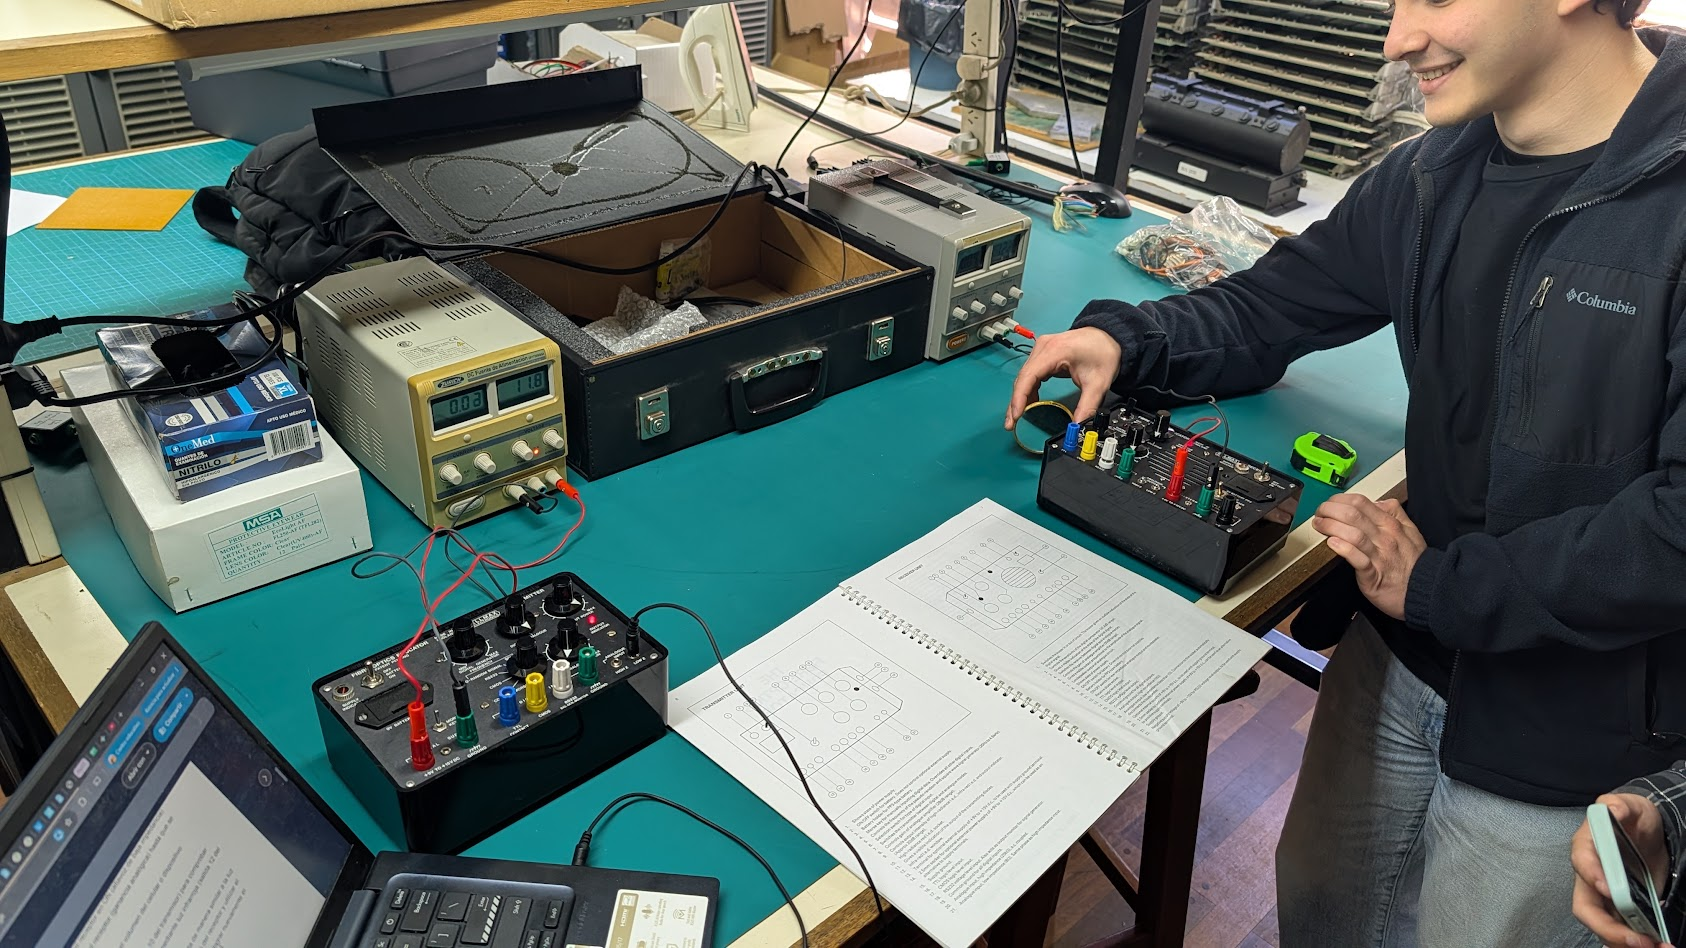
\includegraphics[width=1\textwidth]{espejo.png}}
   \caption{Disposición para la transmisión en espacio libre y reflexión con espejo.}
   \label{fig:espejo}
\end{figure}


\subsubsection{Práctico A.2: Transmisión de Señal de Audio por Fibra Óptica}

\subsubsection*{Consignas y Procedimiento}
\begin{enumerate}
    \item Configurar los modos y potenciómetros iniciales según los pasos 1 a 7 del práctico anterior.
    \item Reproducir audio a volumen casi mínimo e ingresar la señal por el borne 21 del transmisor.
    \item Interconectar la salida óptica 10 del transmisor con la entrada 12 del receptor mediante el cable óptico corto.
    \item Encender el altavoz del receptor (interruptor 11 en ON).
    \item Ajustar levemente el volumen de entrada si la señal resulta muy tenue.
    \item Reducir la potencia del transmisor (potenciómetro 9) para evitar la saturación del fotodetector y eliminar la distorsión.
    \item Ajustar la ganancia del receptor (potenciómetro 5) al nivel de audición óptimo.
    \item Desconectar la fibra del receptor, conectar la fibra larga a este último y enfrentar manualmente los extremos de ambas fibras para verificar el acoplamiento y la continuidad de la señal.
    \item Demostración del emisor indicador: Configurar la máxima potencia en TX y RX, conectar el cable corto al receptor y colocar su extremo libre cerca del LED indicador de salida (LED 11) del transmisor.
\end{enumerate}

\subsubsection*{Resultados, Fotografías y Observaciones}

La transmisión por fibra óptica demostró ser capaz de concentrar una mayor cantidad de potencia hasta el receptor tal que, con la misma configuración de volúmenes que en el práctico anterior, la señal audible se escucha mucho más fuerte.

Por otro lado, al desconectar la fibra y enfrentar de forma manual los conectores, logra escucharse la señal, con un nivel mayor al del práctico anterior, pero no tan alto como con los cables conectados correctamente.

Esto sucede porque en el espacio libre la luz sufre de atenuación geométrica, el haz diverge y la potencia decae con la distancia. En cambio, la fibra óptica confina el haz de luz mediante reflexión total interna, guiando casi toda la potencia óptica emitida directamente hacia el área activa del fotodetector, minimizando las pérdidas. Lo mismo con el caso donde se utilizó el LED indicador para transmitir la información.

\begin{figure}[H]
  \centering
  \begin{subfigure}{0.48\linewidth}
    \fbox{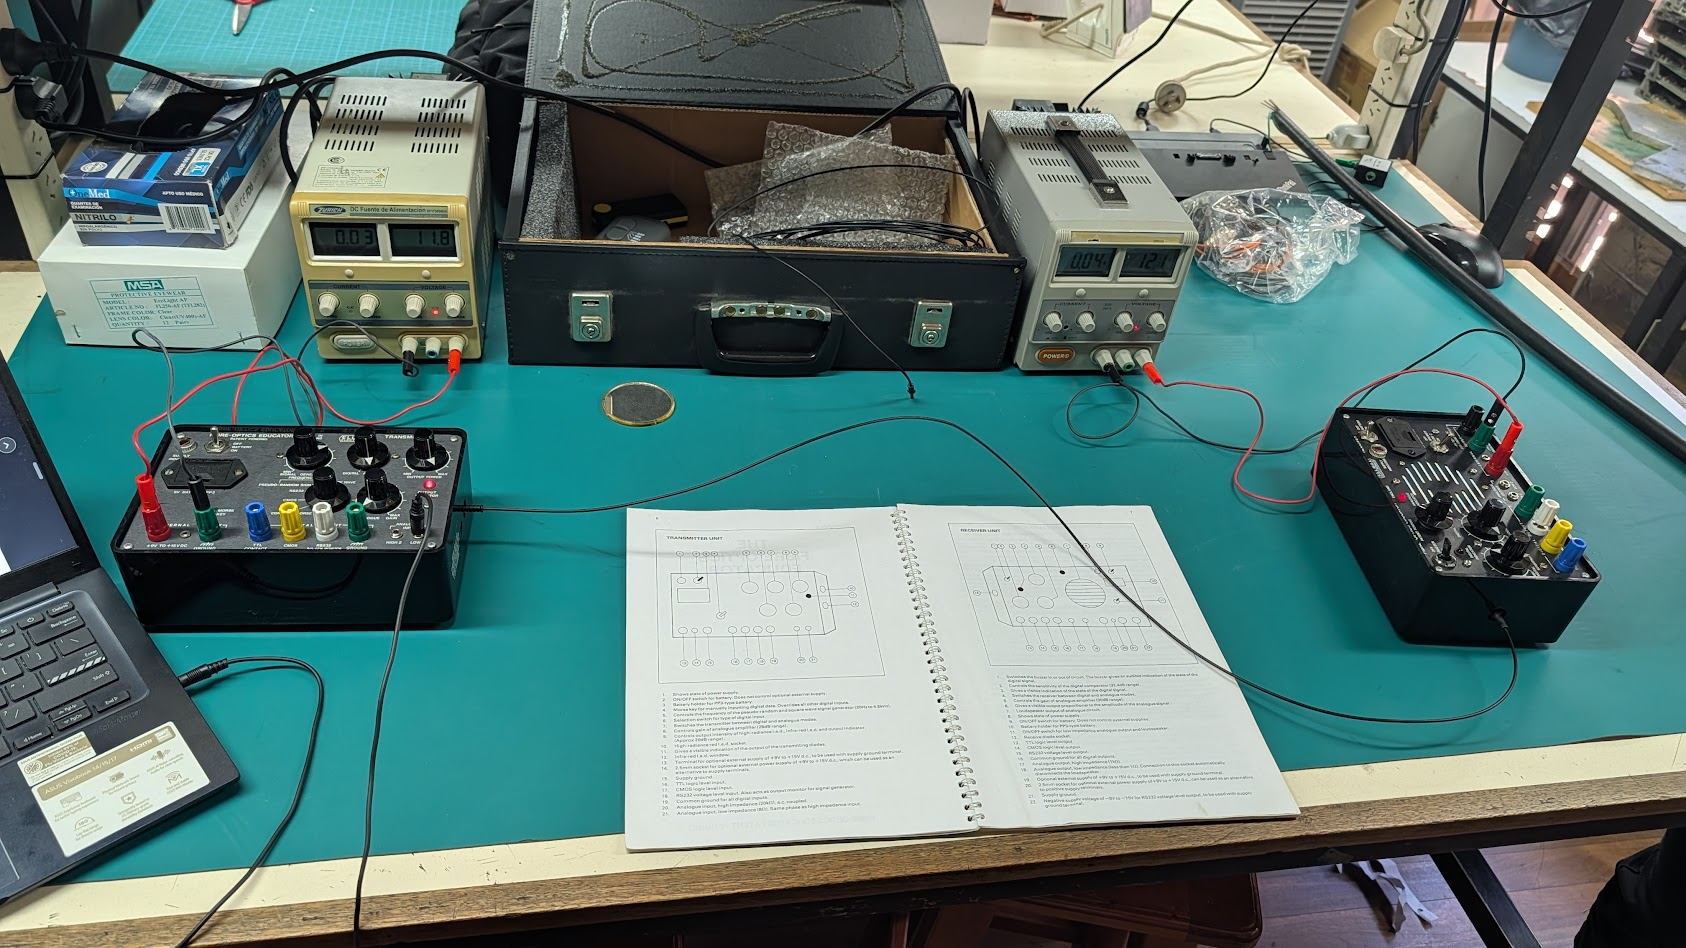
\includegraphics[width=\linewidth]{A2_corto.png}}
    \caption{Práctico con cable de F.O. corto}
    \label{fig:corto}
  \end{subfigure}
  \hfill
  \begin{subfigure}{0.48\linewidth}      
    \fbox{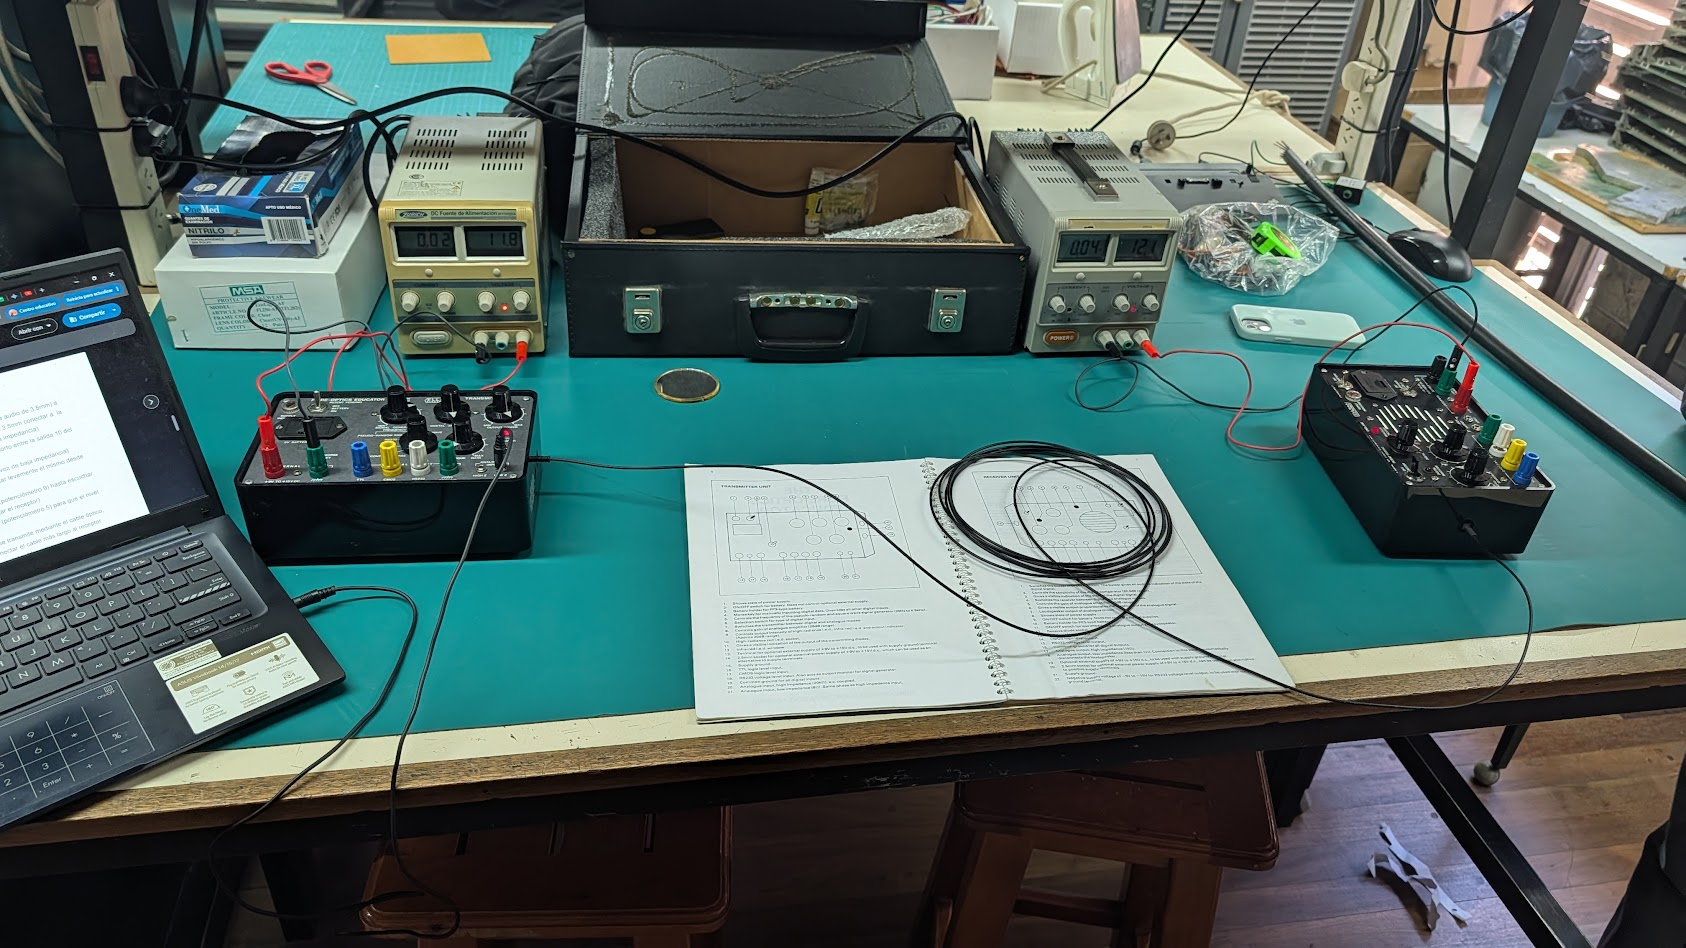
\includegraphics[width=\linewidth]{A2_largo.png}}
    \caption{Práctico con cable de F.O. largo}
    \label{fig:largo}
  \end{subfigure}
  \begin{subfigure}{0.48\linewidth}      
    \fbox{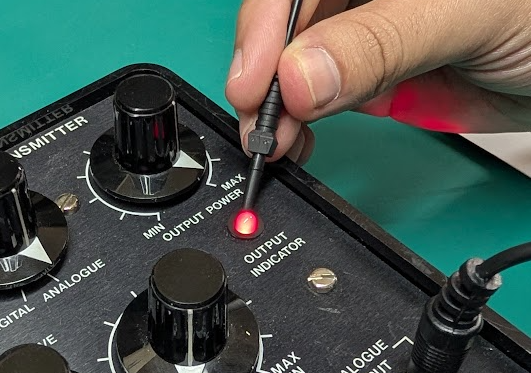
\includegraphics[width=\linewidth]{salida.png}}
    \caption{Extremo del cable enfrentado al LED indicador}
    \label{fig:salida}
  \end{subfigure}
  \hfill
  \begin{subfigure}{0.48\linewidth}      
    \fbox{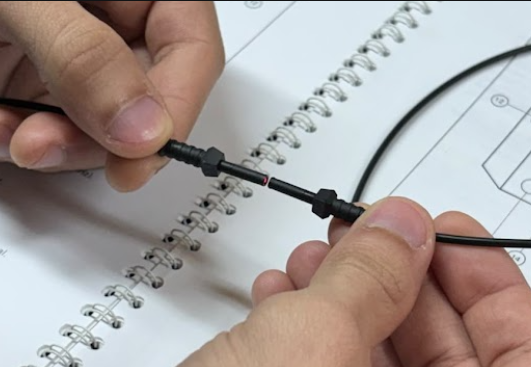
\includegraphics[width=\linewidth]{1.png}}
    \caption{Extremos de cables enfrentados entre sí}
    \label{fig:1}
  \end{subfigure}
  \caption{Imágenes de práctico A.2.}
  \label{fig:A2}
\end{figure}



\subsection{Práctico D: Modo Digital}

\subsubsection{Materiales Necesarios}
\begin{itemize}
    \item Fuente de alimentación (\autoref{fig:alimentacion}).
    \item Cables banana-cocodrilo (\autoref{fig:coco}).
    \item Módulo Transmisor y Módulo Receptor del Kit (\autoref{fig:kit}).
    \item Cable óptico corto y cable óptico largo (\autoref{fig:kit}).
    \item Osciloscopio (\autoref{fig:osc}).
\end{itemize}

\subsubsection{Práctico D.1: Comunicaciones Digitales (Morse y Generador de Ondas)}

\subsubsection*{Consignas y Procedimiento}
\begin{enumerate}
    \item Configurar el transmisor en modo digital (interruptor 7).
    \item Seleccionar la posición TTL CONTACT/MORSE en el interruptor 6 del transmisor.
    \item Ajustar la potencia de salida al máximo (potenciómetro 9).
    \item Seleccionar modo digital en el receptor (interruptor 4).
    \item Ajustar el control de umbral digital (potenciómetro 2 del receptor) en posición intermedia.
    \item Encender el buzzer del receptor (interruptor 1).
    \item Conectar el cable óptico corto entre la salida 10 (TX) y la entrada 12 (RX).
    \item Conectar la fuente de alimentación externa a ambos equipos según el Anexo \ref{Anexo1}.
    \item Presionar el pulsador Morse (interruptor 4 del transmisor) para verificar la emisión.
    \item Desconectar la fibra del transmisor y generar señales digitales utilizando la luz ambiente, modulando la recepción mediante el ajuste del umbral (potenciómetro 2).
    \item Reconectar la fibra óptica y fijar la frecuencia del generador interno del transmisor al mínimo (potenciómetro 5).
    \item Cambiar el interruptor 6 del transmisor a la posición PSEUDO-RANDOM SIGNAL e incrementar progresivamente la frecuencia.
    \item Seleccionar la posición SQUARE WAVE en el interruptor 6.
    \item Variar la frecuencia con el potenciómetro 5 y comprobar el cambio de tono en el altavoz/buzzer del receptor.
    \item Aumentar la frecuencia hasta que la respuesta visual del LED indicador 11 deje de percibir el parpadeo, mientras que el tono acústico continúe variando.
\end{enumerate}

\subsubsection*{Resultados, Fotografías y Observaciones}

Luego de verificar la emisión de información con el pulsador Morse correctamente, se procedió a ajustar el umbral hasta lograr recibir las señales utilizando la luz del ambiente como medio transmisor.

Luego se utilizaron las funciones de PSEUDO-RANDOM SIGNAL y SQUARE WAVE para recibir distintos tipos de señal y con el buzzer pudo escucharse el sonido de dichas señales. Al aumentar la frecuencia, fue posible notar como aumenta el tono que se escucha desde el buzzer, y el parpadeo del LED indicador deja de notarse y pasa a ser una luz constante para el ojo humano.


\subsubsection{Práctico D.2: Mediciones en Funcionamiento Digital}

\subsubsection*{Consignas y Procedimiento}
\begin{enumerate}
    \item Configurar los modos y potenciómetros iniciales según los pasos 1 a 8 del práctico anterior
    \item Seleccionar la posición SQUARE WAVE en el interruptor 6.
    \item Conectar un osciloscopio conectado en los bornes RS232 (blancos) y GROUND (verdes) en el transmisor y receptor. 
    \item Comparar la onda emitida por el transmisor y la onda de salida del receptor en modo digital con el generador de onda cuadrada.
    \item Comparar frecuencias, ancho de banda (para todo el rango de frecuencia de trabajo del generador) y amplitudes. 
    \item Verificar si la onda del transmisor se encuentra en fase con el receptor y si existe o no inversión de la misma. 
    \item Observar que ocurre al variar los potenciómetros 9 y 2 del transmisor y receptor respectivamente (potencia de salida y umbral digital).
    \item Demostrar con el ajuste de los mismos que la atenuación del cable óptico largo es mayor a la del corto.
\end{enumerate}

\subsubsection*{Resultados, Fotografías y Observaciones}

Se lograron ver las curvas de entrada y salida, en fase entre ellas, sin embargo, con la función de ``Medidas'' del osciloscopio logra notarse una amplificación de la señal que se atribuye a que el modo digital lleva la señal de salida al valor de la tensión de alimentación.

Las frecuencias extremas de operación (20,64 Hz en el límite inferior y 4,745 kHz en el superior, ver \autoref{fig:inferior} y \autoref{fig:superior}) generan deformaciones en la onda cuadrada que evidencian las limitaciones en la respuesta en frecuencia del circuito. En el límite inferior, se observa una caída en los niveles de tensión constante, lo que corresponde a un efecto de acoplamiento en AC (filtro pasa-altos), atribuido a que los canales del osciloscopio están configurados en Acoplamiento AC, y el capacitor de bloqueo de DC puede generar la atenuación en la parte plana de las curvas a frecuencias bajas. Por el contrario, en el límite superior, los flancos pierden verticalidad y se observan redondeados, un efecto de filtro pasa-bajos que es consecuencia directa de la capacitancia intrínseca del circuito interactuando con la resistencia de carga, lo que limita la velocidad de respuesta del sistema y aumenta los tiempos de conmutación.

La \autoref{fig:umbral} es consecuencia de setear el umbral en el límite donde recibe la señal con el cable óptico corto, tal que al cambiar al cable óptico largo el aumento de atenuación hace que la señal no pase el umbral y en consecuencia no haya señal a la salida.


\begin{figure}[H]
  \centering
  \begin{subfigure}{0.42\linewidth}
    \fbox{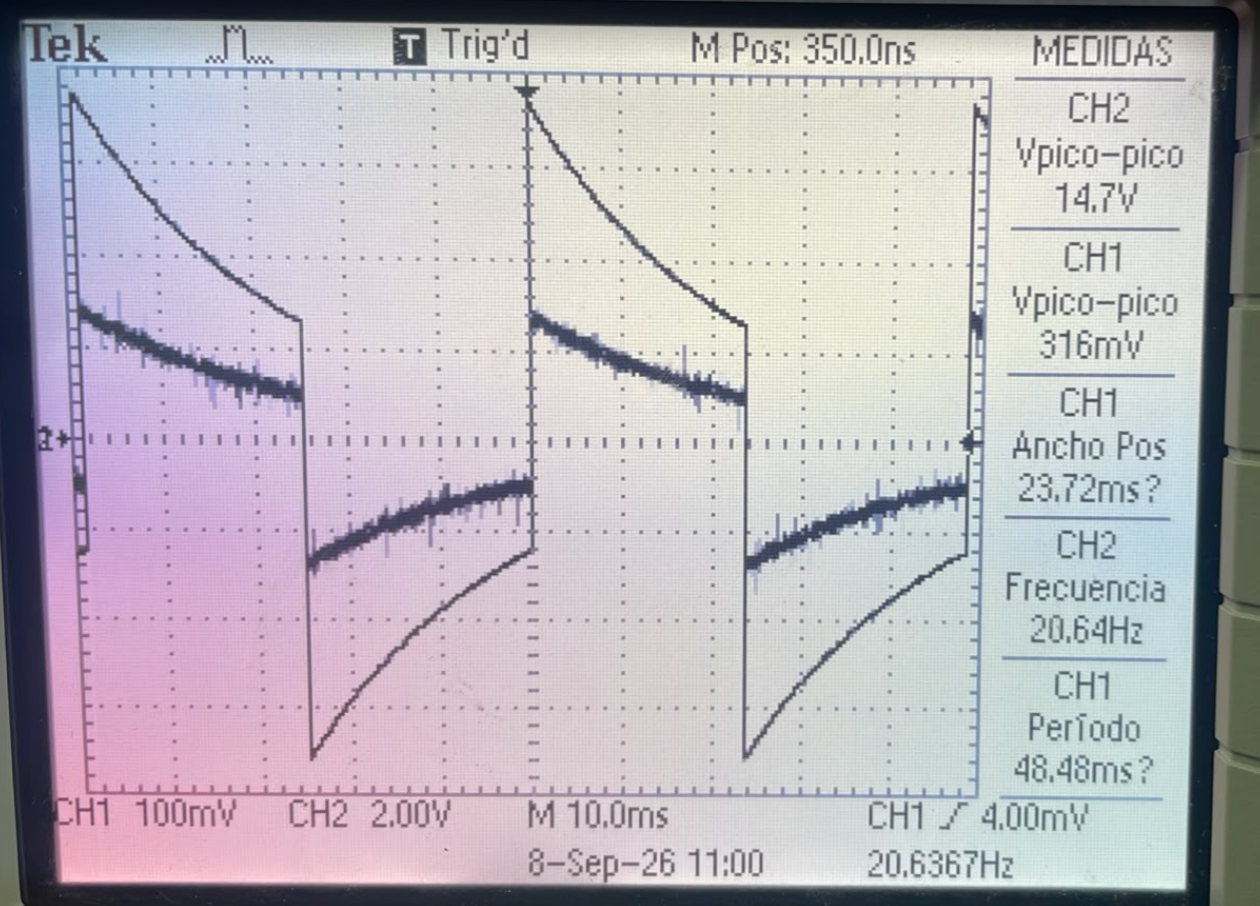
\includegraphics[width=\linewidth]{20hz.png}}
    \caption{Límite inferior de frecuencia.}
    \label{fig:inferior}
  \end{subfigure}
  \hfill
  \begin{subfigure}{0.53\linewidth}      
    \fbox{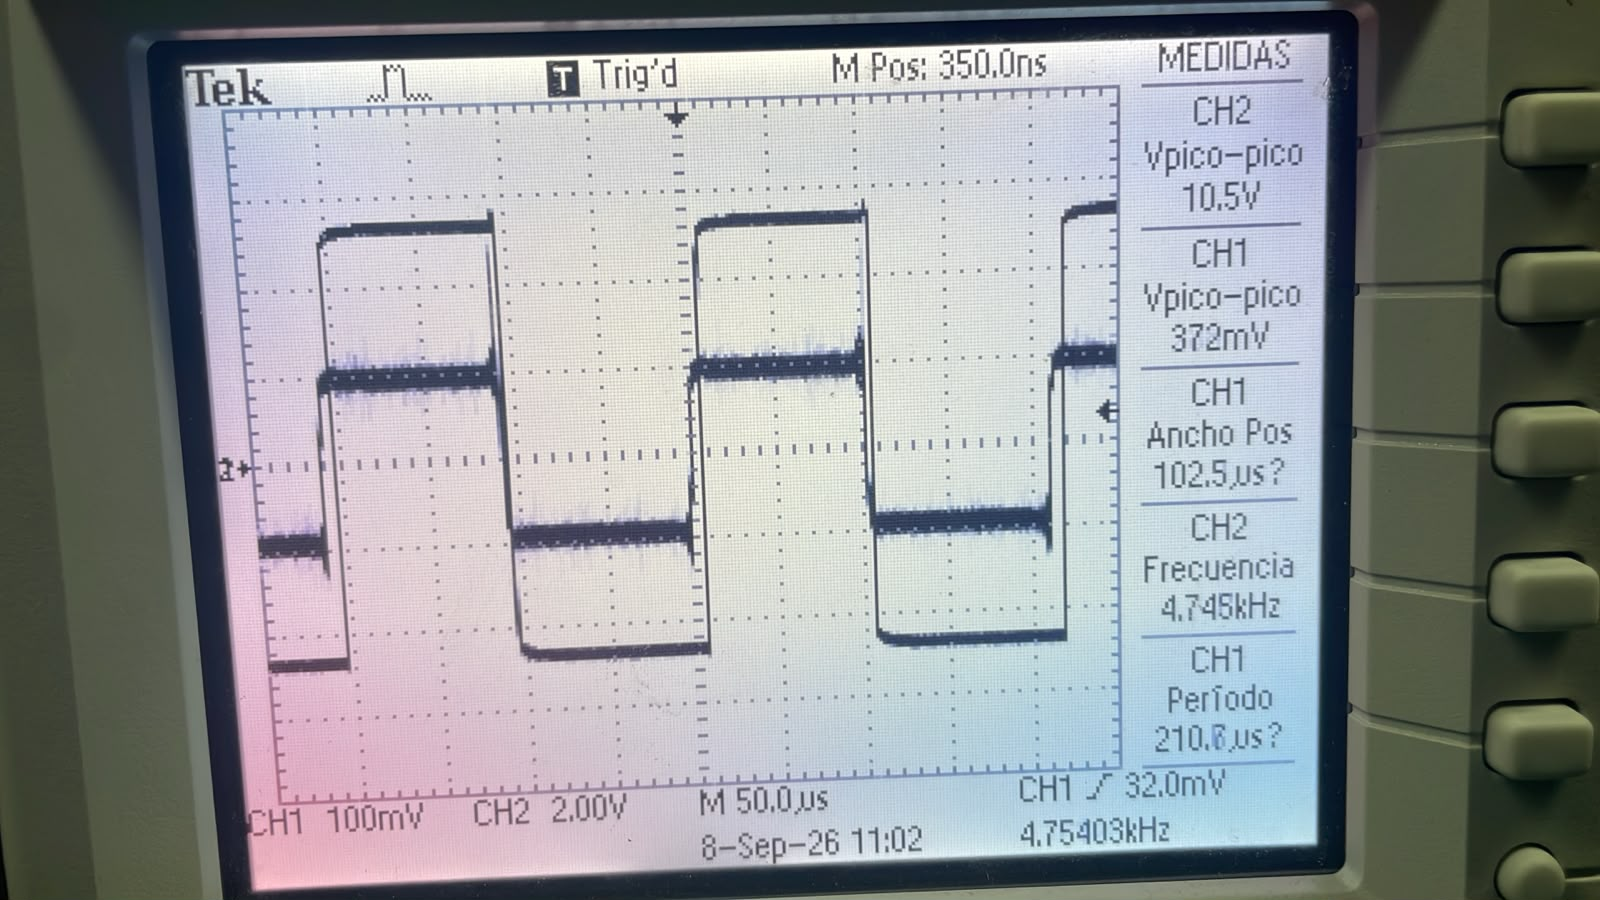
\includegraphics[width=\linewidth]{4khz.png}}
    \caption{Límite superior de frecuencia.}
    \label{fig:superior}
  \end{subfigure}
  \begin{subfigure}{0.55\linewidth}      
    \fbox{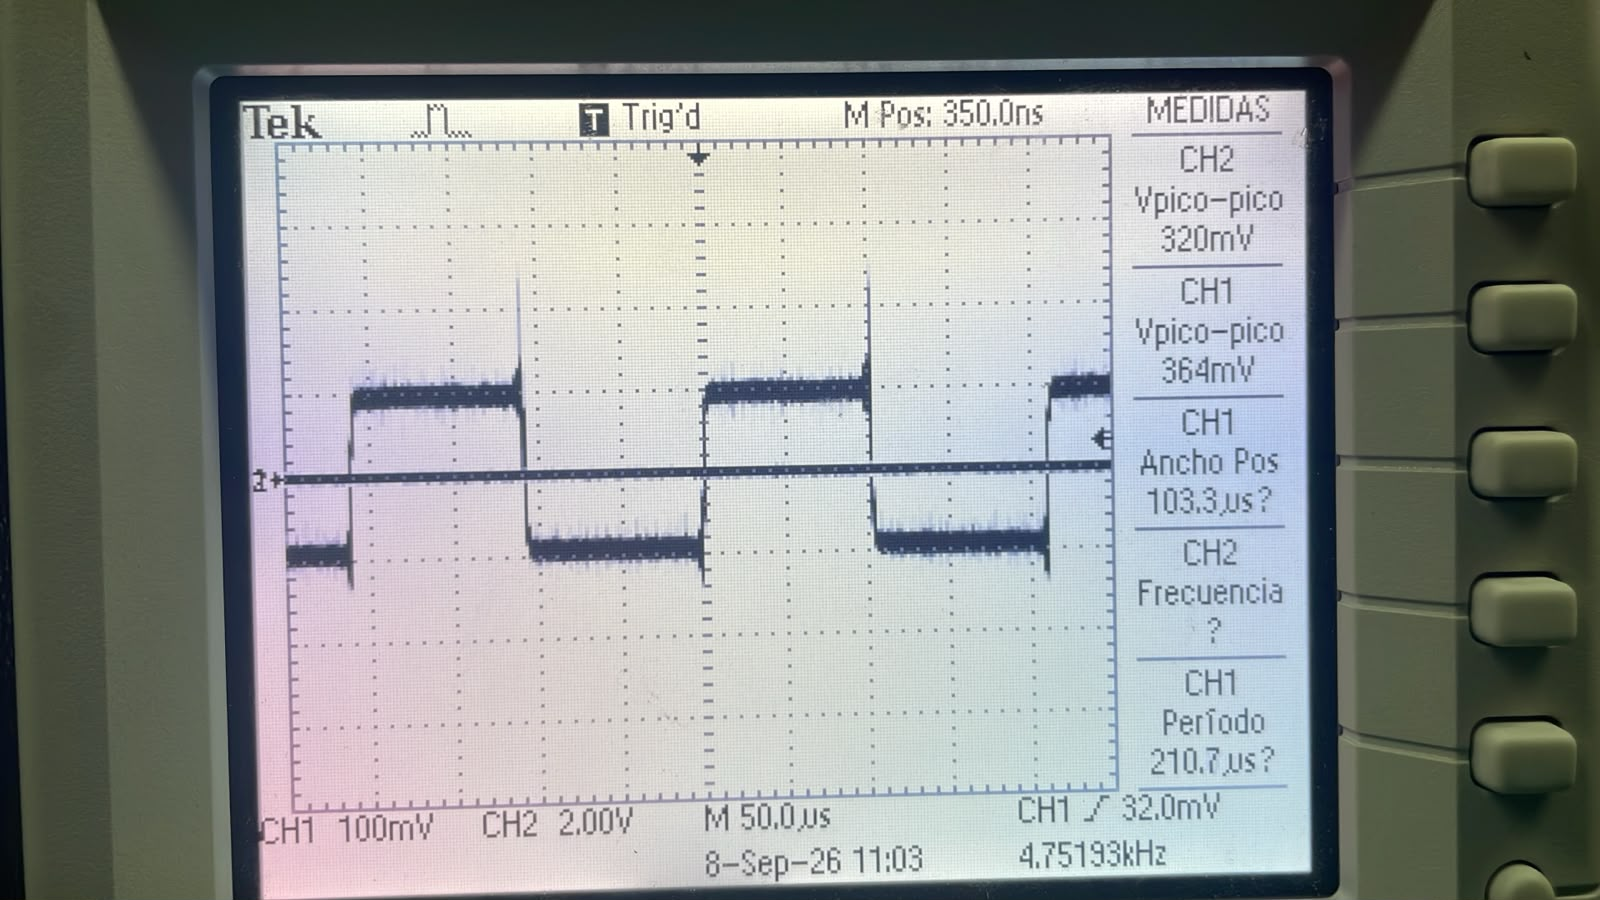
\includegraphics[width=\linewidth]{umbral.png}}
    \caption{Entrada y Salida con cable óptico largo.}
    \label{fig:umbral}
  \end{subfigure}
  \caption{Imágenes de Práctico D.2.}
  \label{fig:D2}
\end{figure}

\subsection{Conclusiones - Parte 1}

Se demostró la superioridad de la propagación guiada por fibra óptica frente a la transmisión en espacio libre. Mientras que en el espacio libre la divergencia del haz lumínico genera una rápida atenuación y exige una alineación estricta entre emisor y receptor, la fibra óptica logra confinar la energía mediante el fenómeno de reflexión total interna, garantizando que una fracción mayor de la potencia óptica emitida incida sobre la zona activa del fotodetector, mejorando drásticamente la relación señal a ruido y el nivel de la señal recuperada.

El análisis del modo digital evidenció el comportamiento de los transmisores y receptores adaptados a normativas de comunicación de datos (como RS232). Se corroboró que el sistema receptor no opera de forma lineal, sino como un comparador lógico que conmuta su salida a los niveles de la tensión de alimentación una vez que la señal óptica supera el umbral preestablecido. 

Asimismo, se verificó el impacto crítico de la atenuación del medio en los sistemas digitales: al incrementar la longitud de la fibra, las pérdidas intrínsecas aumentan, reduciendo la potencia recibida. Si esta potencia cae por debajo del umbral de decisión, el receptor es incapaz de regenerar el pulso, evidenciando que un correcto balance del enlace (potencia de emisión vs. sensibilidad y umbral de recepción) es vital para mantener la comunicación.

\newpage

\section{Parte 2: Herramientas para Instalación de Fibra Óptica}

\subsection{Materiales Necesarios}
\begin{itemize}
    \item Localizador visual de fallas (VFL - \textit{Visual Fault Locator}) (\autoref{fig:vfl}).
    \item Tramo de cable óptico, \textit{pigtail} o \textit{patchcord} a inspeccionar.
    \item Contenedor seguro para desecho de fibra y kit de limpieza (alcohol isopropílico y paños).
    \item Medidor de potencia óptica (\autoref{fig:medidor})
    \item Conector mecánico rápido SC-APC (\autoref{fig:sc_apc}).
    \item Cable de fibra óptica a conectorizar.
    \item Pinza peladora de precisión (\autoref{fig:stripper}).
    \item Cortadora de precisión para fibra óptica (\autoref{fig:cortadora}).
    \item Herramienta de montaje 3M Fibrlok II Assembly Tool 2501 (\autoref{fig:herramienta}).
    \item Módulos de empalme mecánico (\autoref{fig:empalmes_mecanicos}).
    \item Cables de fibra óptica a empalmar.
\end{itemize}


\subsection{Práctico A: Detección Visual de Fallas}

\subsubsection*{Consignas y Procedimiento}
\begin{enumerate}
    \item Acoplar el localizador visual de fallas (VFL) al conector de entrada del tramo de fibra óptica bajo prueba.
    \item Encender la fuente láser del VFL en modo de emisión continua o pulsada.
    \item Inspeccionar a lo largo de la cubierta del cable y en el extremo opuesto la presencia de luz roja visible para identificar el núcleo, así como roturas internas, macrocurvaturas excesivas o fisuras.
    
\end{enumerate}

\subsubsection*{Resultados, Fotografías y Observaciones}

La prueba mediante el localizador visual de fallas (VFL) permitió comprobar la continuidad óptica del hilo de fibra. En un tramo en buen estado, la luz roja visible se proyecta como un punto brillante definido en el extremo distante sin fugas laterales. 

Adicionalmente, se intentó cuantificar la potencia del haz mediante un medidor de potencia óptica, tal como se aprecia en la \autoref{fig:monja}. Sin embargo, la fuente VFL opera a una longitud de onda de $650\text{ nm}$, mientras que la longitud de onda mínima seleccionable en el medidor es de $800\text{ nm}$. Dado que la capacidad de respuesta del sensor interno del instrumento depende intrínsecamente de $\lambda$, la calibración para $800\text{ nm}$ introduce un error de escala en la lectura. Si bien la medición arrojó un valor distinto de cero (lo que permite confirmar cualitativamente la presencia y continuidad de la señal óptica), la magnitud desplegada no resulta cuantitativamente precisa.

\begin{figure}[H]
  \centering
  \fbox{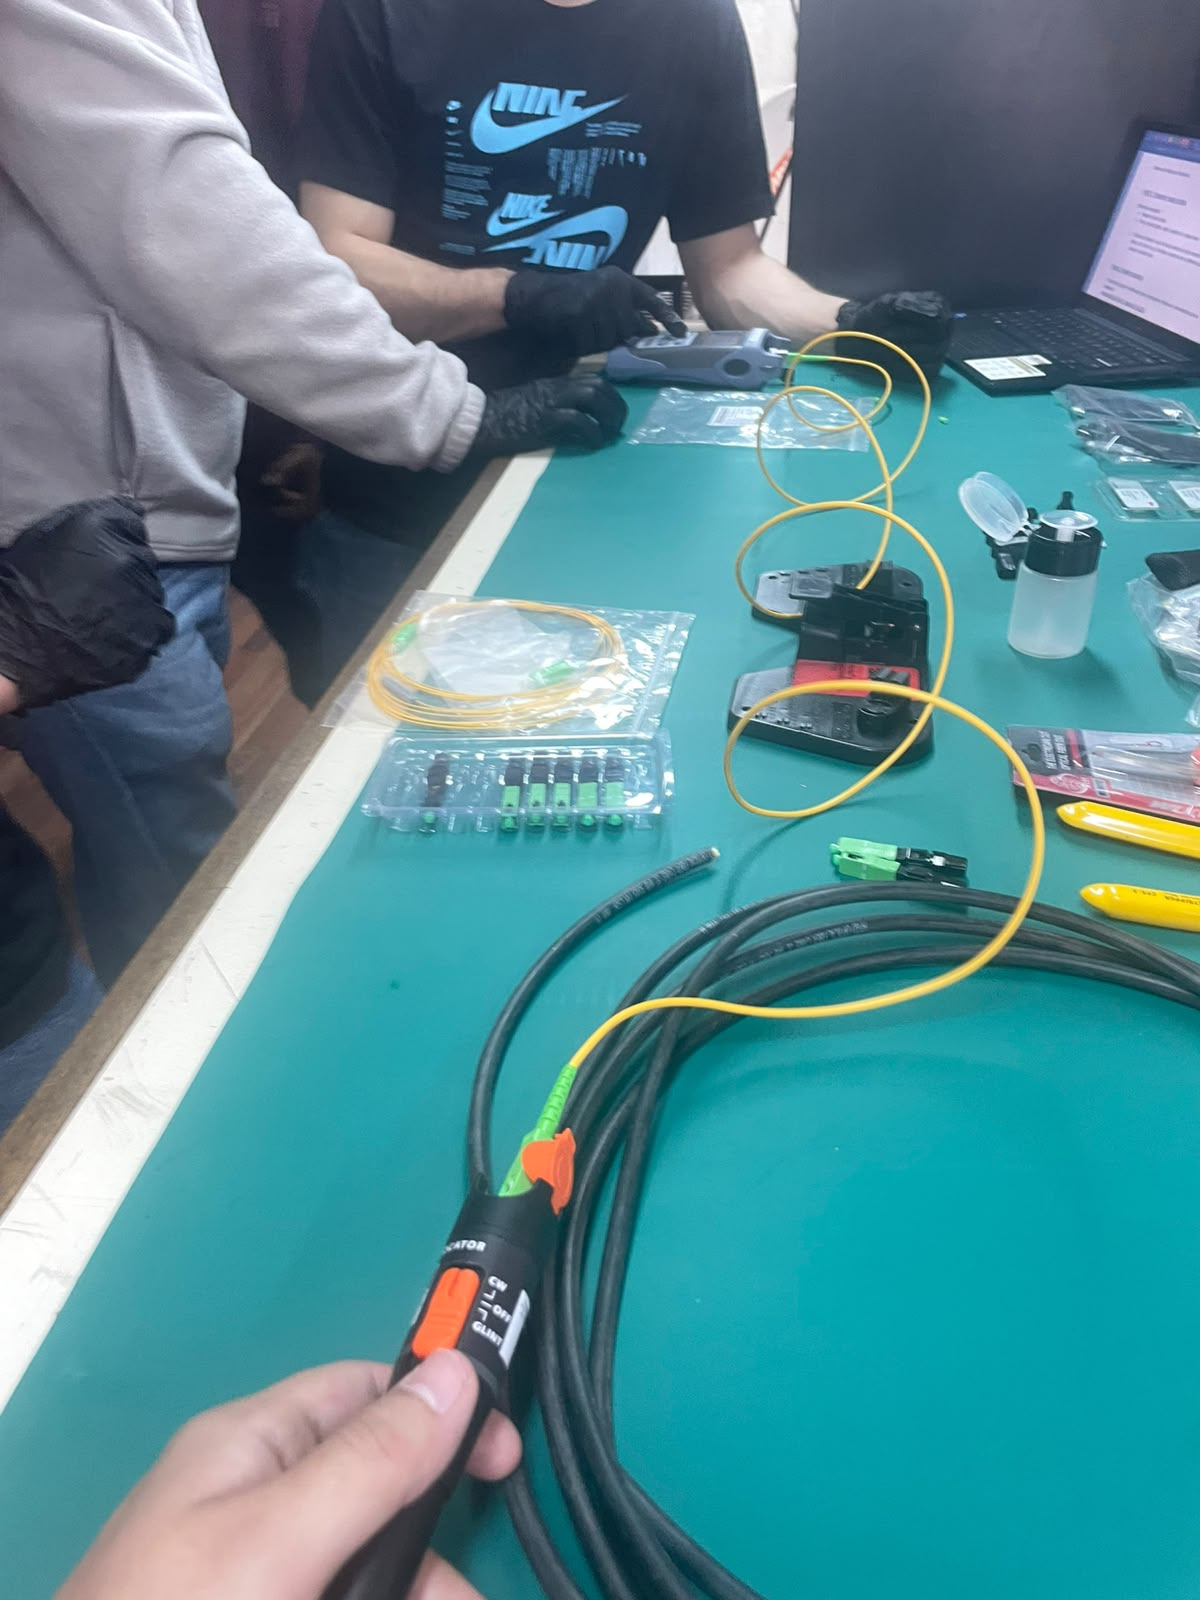
\includegraphics[width=0.35\textwidth]{monja.png}}
  \caption{Inspección visual de continuidad y detección de fallas mediante VFL.}
  \label{fig:monja}
\end{figure}

\subsection{Práctico B: Conectorización Mecánica de Fibra Óptica}

\subsubsection*{Consignas y Procedimiento}
\begin{enumerate}
    \item Desarmar las piezas principales del conector mecánico SC-APC.
    \item Retirar aproximadamente $40\,\text{mm}$ de la cubierta exterior del cable e introducir la bota a rosca del conector.
    \item Pelar la fibra manteniendo $20\,\text{mm}$ de recubrimiento secundario.
    \item Limpiar la fibra expuesta con un paño embebido en alcohol isopropílico.
    \item Cortar la fibra a una longitud exacta de $10\,\text{mm}$ utilizando la cortadora de precisión.
    \item Verificar que la traba/seguro naranja del conector se encuentre retrotraído.
    \item Insertar la fibra en el conector hasta sentir el tope y observar la formación de un ligero arco de control.
    \item Fijar la fibra deslizando el seguro naranja hacia adelante.
    \item Deslizar ligeramente la fibra hacia atrás para quitar el arco y dejarla recta.
    \item Roscar la bota posterior y colocar la carcasa protectora externa del conector SC-APC.
\end{enumerate}

\subsubsection*{Resultados, Fotografías y Observaciones}

Luego de varios intentos en los que se quebraba la fibra debido a la inexperiencia con las herramientas, la conectorización con conectores mecánicos SC-APC demostró ser una técnica eficiente.

Durante el procedimiento, la formación del arco de control confirmó que la fibra recortada hace contacto físico continuo contra el tope interno. Sin embargo, al momento de la medición con el medidor de potencia, éste marcó que no recibía potencia.

\begin{figure}[H]
  \centering
  \begin{subfigure}{0.32\linewidth}
    \fbox{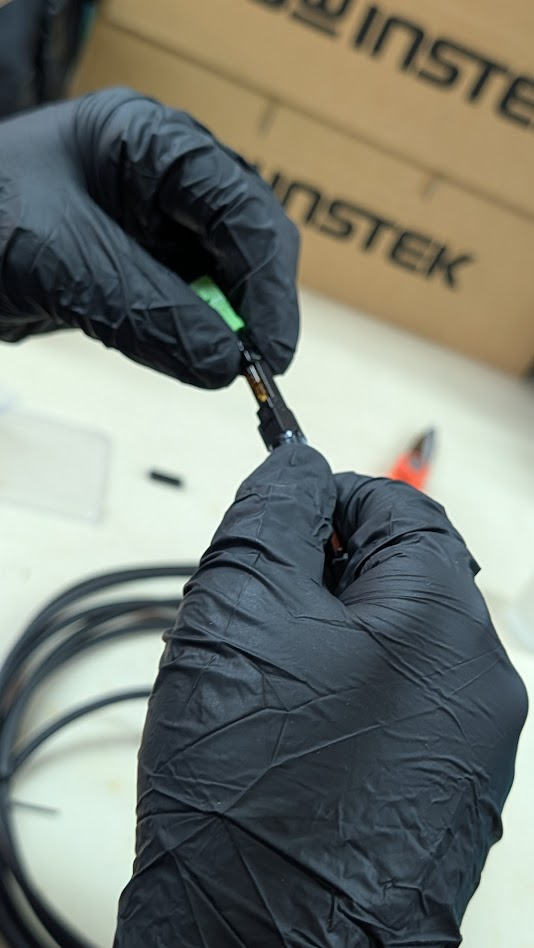
\includegraphics[width=\linewidth]{cris.png}}
    \caption{Inserción de la fibra recortada en el conector.}
    \label{fig:cris}
  \end{subfigure}
  \hfill
  \begin{subfigure}{0.48\linewidth} 
    \fbox{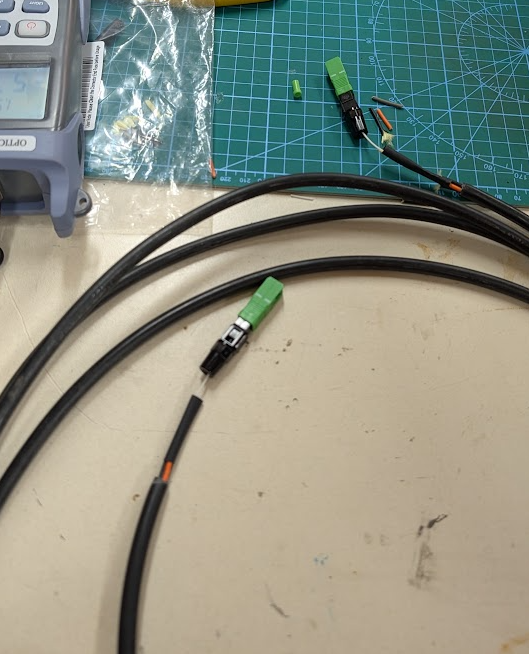
\includegraphics[width=\linewidth]{conector.png}}
    \caption{Conector SC-APC armado y bloqueado.}
    \label{fig:conector}
  \end{subfigure}
  \caption{Proceso de montaje de conector rápido SC-APC.}
  \label{fig:practico_a}
\end{figure}

\subsection{Práctico C: Empalme Mecánico de Fibra Óptica}

\subsubsection*{Consignas y Procedimiento}
\begin{enumerate}
    \item Colocar un módulo de empalme en la cuna de la herramienta de montaje 2501 presionando firmemente los extremos.
    \item Orientar los brazos de retención con almohadillas según el diámetro de recubrimiento de las fibras ($250\,\mu\text{m}$ o $900\,\mu\text{m}$).
    \item Pelar entre $25\,\text{mm}$ y $51\,\text{mm}$ del recubrimiento de la primera fibra dejando el vidrio expuesto.
    \item Limpiar la fibra desnuda con un paño impregnado en alcohol isopropílico.
    \item Efectuar el corte de precisión con la cortadora de precisión a $12.5\,\text{mm}$ y verificar la longitud con la escala impresas en la herramienta 2501.
    \item Sujetar la fibra en el brazo de retención e insertarla suavemente en el empalme hasta sentir resistencia, comprobando que quede con un arco máximo de $3\,\text{mm}$.
    \item Preparar (pelar, limpiar y cortar a $12.5\,\text{mm}$) la segunda fibra.
    \item Insertar la segunda fibra por el lado opuesto del empalme hasta encontrar resistencia e igualar los arcos de ambas fibras.
    \item Accionar la palanca de montaje para cerrar la tapa del empalme, fijando mecánicamente la alineación de ambos núcleos con el gel de adaptación de índice de refracción.
    \item Retirar las fibras de las almohadillas de retención y extraer el empalme completado.
\end{enumerate}

\subsubsection*{Resultados, Fotografías y Observaciones}

El empalme permitió lograr un acoplamiento mecánico entre dos tramos de fibra sin necesidad de fusión térmica. La precisión en las etapas de pelado, limpieza minuciosamente ejecutada con alcohol isopropílico y el corte plano mediante la cortadora, resultaron determinantes, y tomaron varios intentos hasta lograr las dimensiones correctas de la fibra para ejecutar el empalme.

Debido a que se utilizó el mismo cable del práctico anterior, el medidor de potencia volvió a marcar que no recibía potencia.

Posteriormente, se agregó una protección al empalme (\autoref{fig:protector}) que permite guardar los segmentos desprotegidos de cable alrededor de un plástico.

\begin{figure}[H]
  \centering
  \begin{subfigure}{0.38\linewidth}
    \fbox{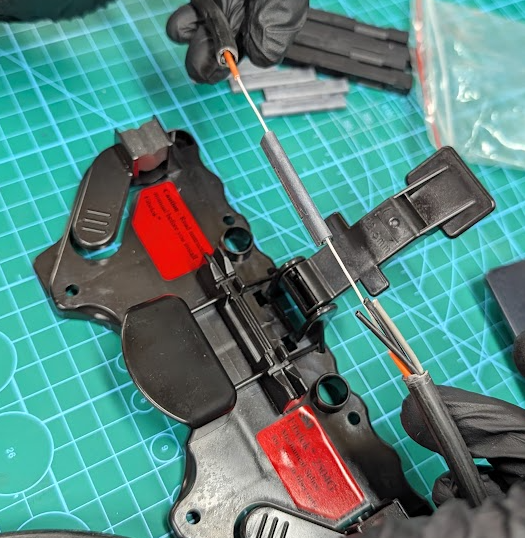
\includegraphics[width=\linewidth]{empalme.png}}
    \caption{Cable empalmado final.}
    \label{fig:empalme_proceso}
  \end{subfigure}
  \hfill
  \begin{subfigure}{0.59\linewidth} 
    \fbox{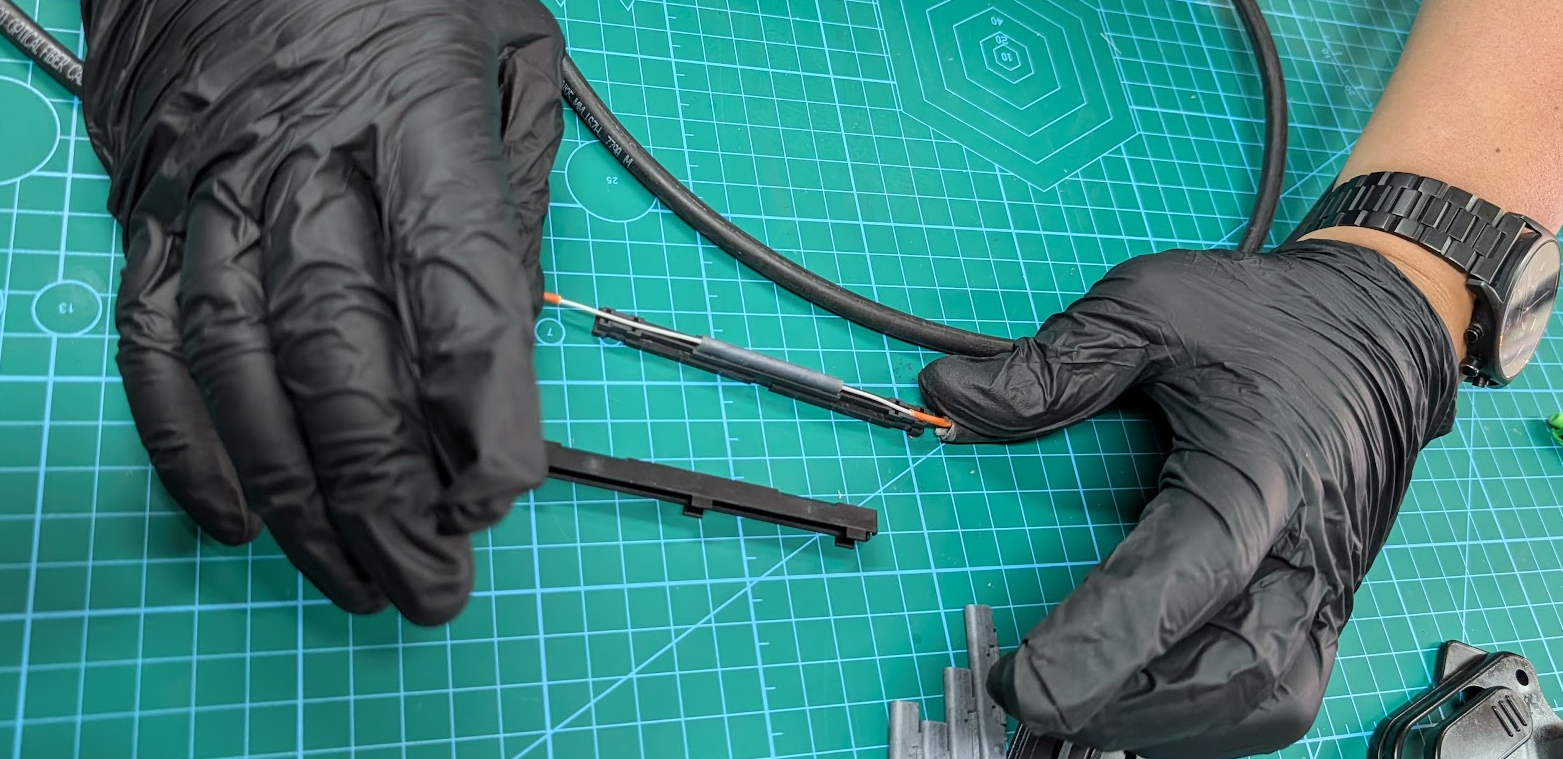
\includegraphics[width=\linewidth]{proteccion.png}}
    \caption{Empalme con protector.}
    \label{fig:empalme_completado}
  \end{subfigure}
  \caption{Procedimiento de ejecución del empalme mecánico.}
  \label{fig:empalme_mecanico}
\end{figure}



\subsection{Conclusiones - Parte 2}

La realización de esta segunda parte evidenció que, si bien los empalmes y conectores mecánicos evitan el uso de costosas fusionadoras, la preparación manual de la fibra exige un alto nivel de precisión. En primer lugar, el localizador visual de fallas (VFL) demostró ser una herramienta de diagnóstico clave para verificar la continuidad y detectar fugas de luz por fisuras a simple vista. 

Por otro lado, los inconvenientes experimentados durante el armado del conector SC-APC y el empalme, que se atribuyen a una rotura de la fibra en algún punto que no se trató con cuidado y se rompió, derivando en una lectura de potencia nula, dejaron en evidencia la extrema fragilidad del material ante manipulaciones bruscas. Este fallo demuestra que no hay margen para errores: una limpieza deficiente, una mínima desviación en la longitud del corte con la cortadora de precisión, o una mala inserción que impida el contacto físico entre los núcleos, son suficientes para atenuar por completo la señal. No pudo ser asegurado el lugar de la rotura mediante el VFL, debido a que el cable poseía varias capas de cobertura, por lo que el haz o el punto de luz en la rotura interna no era visible.

En definitiva, se comprobó empíricamente que el éxito de un enlace óptico depende de una técnica de acondicionamiento rigurosa, ya que cualquier error manual penaliza drásticamente la viabilidad de la transmisión.
\newpage

\appendix

\section{Materiales Utilizados}
\label{Anexo2}


\begin{figure}[H]
  \centering
  \begin{subfigure}{0.38\linewidth}
    \fbox{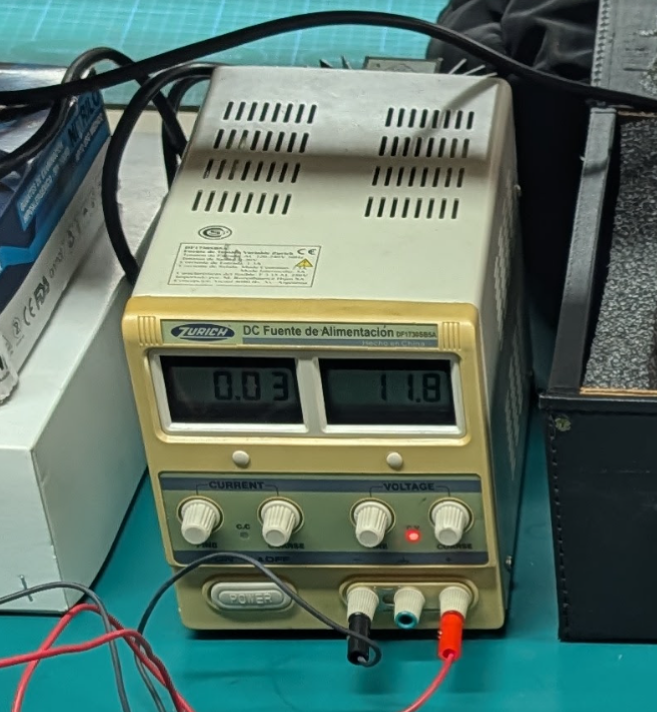
\includegraphics[width=\linewidth]{Alimentacion.png}}
    \caption{Fuente de alimentacion externa}
    \label{fig:alimentacion}
  \end{subfigure}
  \hfill
  \begin{subfigure}{0.42\linewidth}      
    \fbox{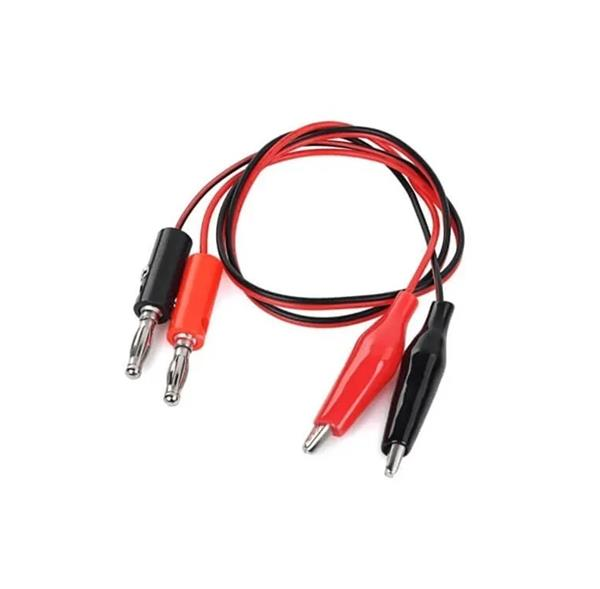
\includegraphics[width=\linewidth]{Coco.png}}
    \caption{Cable banana-cocodrilo}
    \label{fig:coco}
  \end{subfigure}
  \begin{subfigure}{0.44\linewidth}      
    \fbox{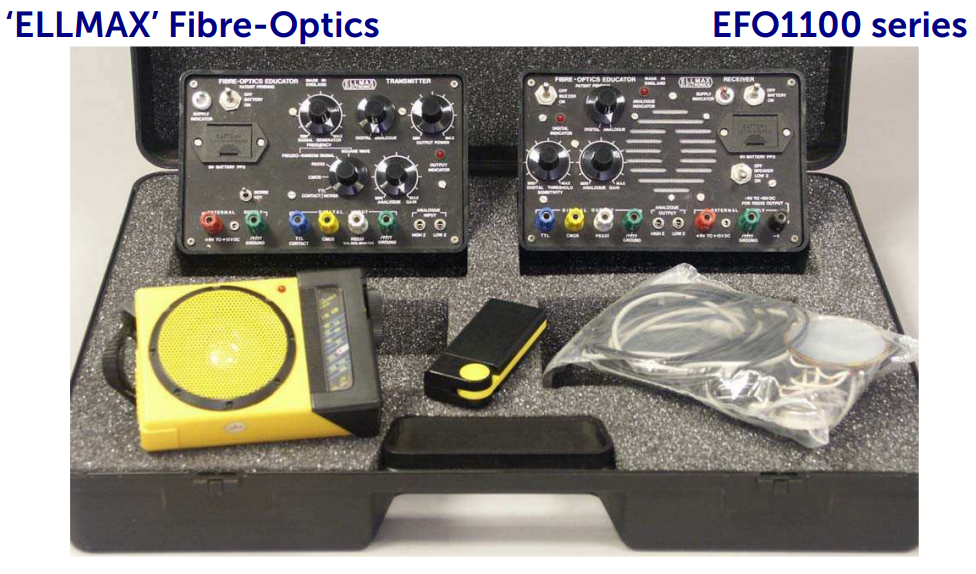
\includegraphics[width=\linewidth]{kit.png}}
    \caption{Kit de Fibra Óptica. Contiene Transmisor, Receptor, Espejo y Cables}
    \label{fig:kit}
  \end{subfigure}
  \hfill
  \begin{subfigure}{0.44\linewidth}      
    \fbox{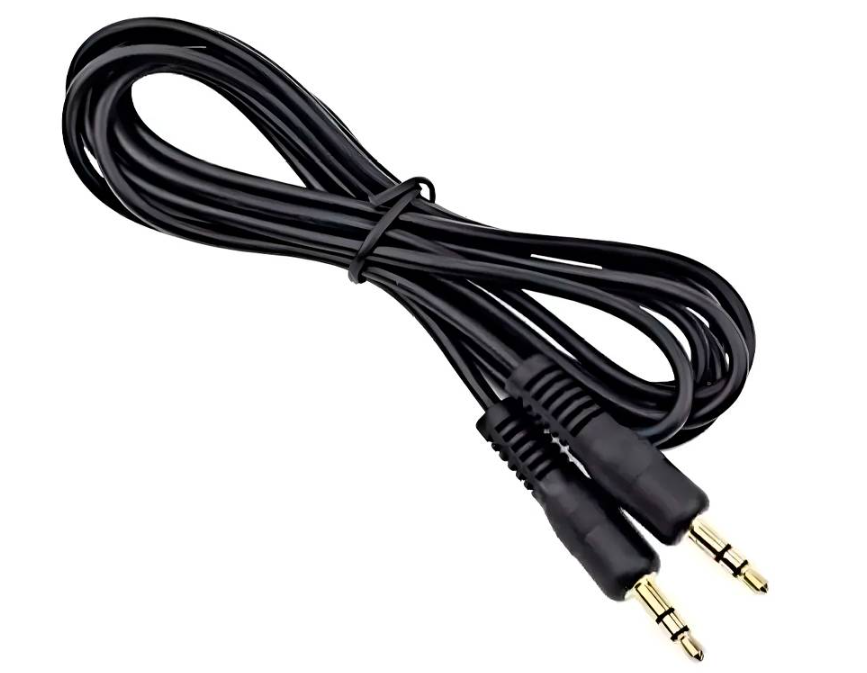
\includegraphics[width=\linewidth]{jack.png}}
    \caption{Cable jack 3,5 mm}
    \label{fig:jack}
  \end{subfigure}
  \begin{subfigure}{0.44\linewidth}      
    \fbox{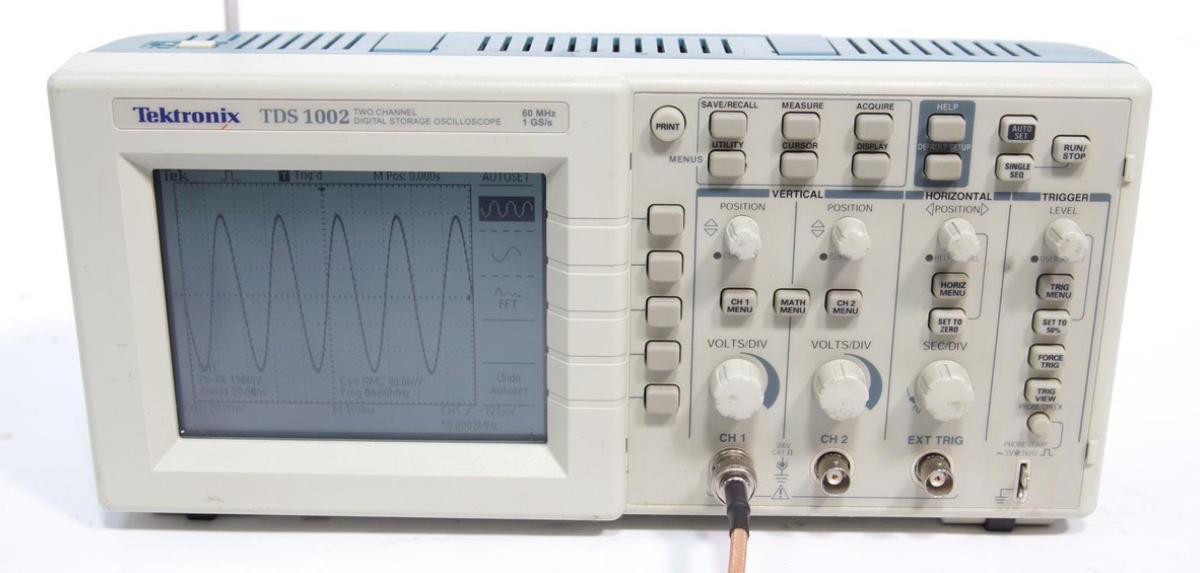
\includegraphics[width=\linewidth]{osc.png}}
    \caption{Osciloscopio Digital Tektronix. Serie TDS.}
    \label{fig:osc}
  \end{subfigure}
  \hfill
  \begin{subfigure}{0.44\linewidth}      
    \fbox{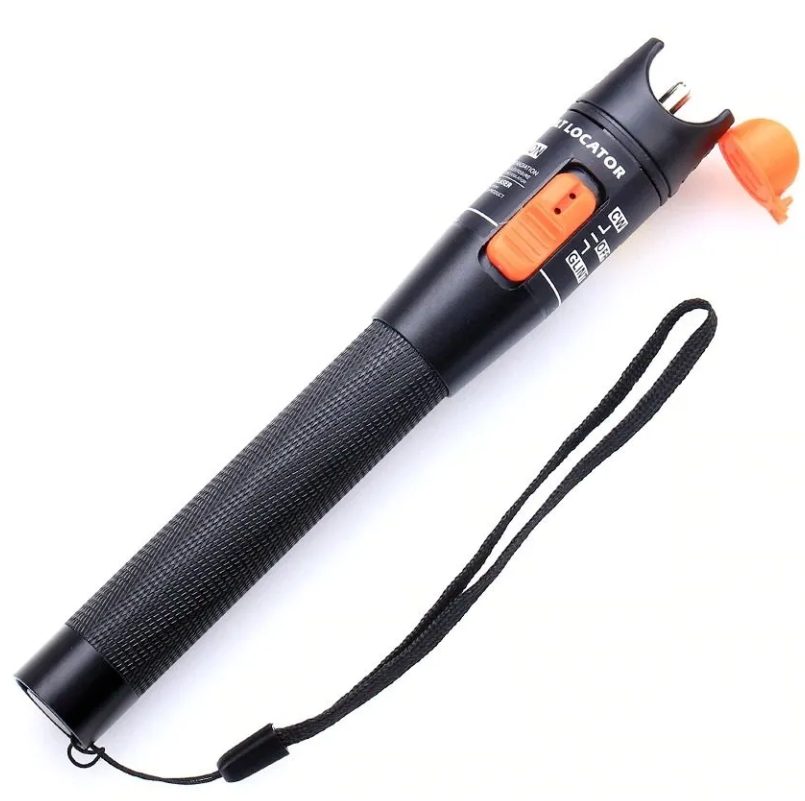
\includegraphics[width=\linewidth]{vfl.png}}
    \caption{Localizador visual de fallas (VFL).}
    \label{fig:vfl}
  \end{subfigure}
  \caption{Materiales Necesarios 1.}
  \label{fig:elementos1}
\end{figure}

\begin{figure}[H]
  \centering
  \begin{subfigure}{0.26\linewidth}      
    \fbox{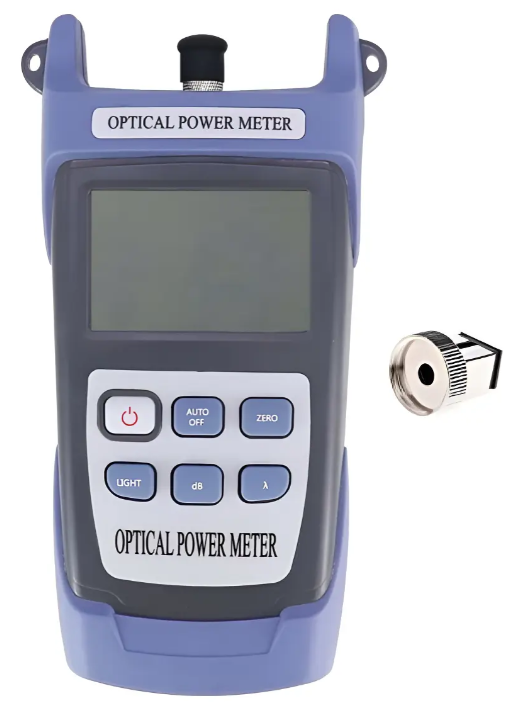
\includegraphics[width=\linewidth]{medidor.png}}
    \caption{Medidor de Potencia Óptica.}
    \label{fig:medidor}
  \end{subfigure}
  \hfill
  \begin{subfigure}{0.4\linewidth}      
    \fbox{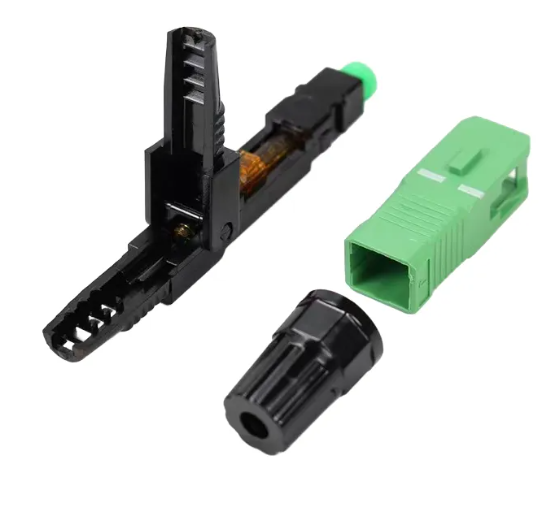
\includegraphics[width=\linewidth]{sc_apc.png}}
    \caption{Conector mecánico SC-APC.}
    \label{fig:sc_apc}
  \end{subfigure}
  \begin{subfigure}{0.44\linewidth}      
    \fbox{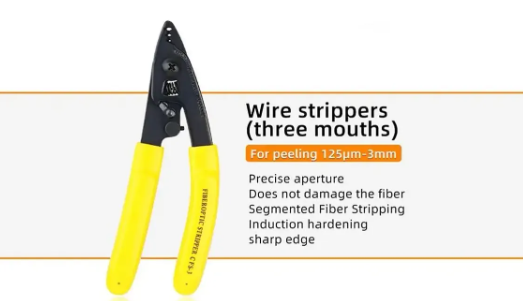
\includegraphics[width=\linewidth]{strippers.png}}
    \caption{Pinza Peladora de Precisión.}
    \label{fig:stripper}
  \end{subfigure}
  \hfill
  \begin{subfigure}{0.44\linewidth}      
    \fbox{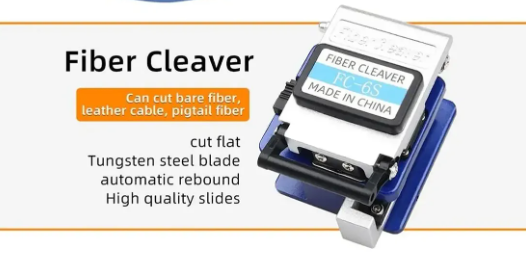
\includegraphics[width=\linewidth]{cortadora.png}}
    \caption{Cortadora de Precisión para Fibra Óptica.}
    \label{fig:cortadora}
  \end{subfigure}
  \begin{subfigure}{0.48\linewidth}      
    \fbox{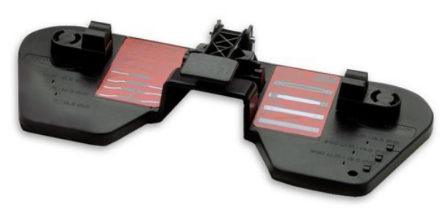
\includegraphics[width=\linewidth]{herramienta.png}}
    \caption{Herramienta 3M Fibrlok II Assembly Tool 2501.}
    \label{fig:herramienta}
  \end{subfigure}
  \hfill
  \begin{subfigure}{0.33\linewidth}      
    \fbox{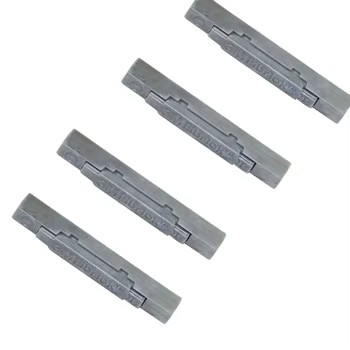
\includegraphics[width=\linewidth]{empalmes.png}}
    \caption{Empalmes mecánicos.}
    \label{fig:empalmes_mecanicos}
  \end{subfigure}
  \begin{subfigure}{0.4\linewidth}      
    \fbox{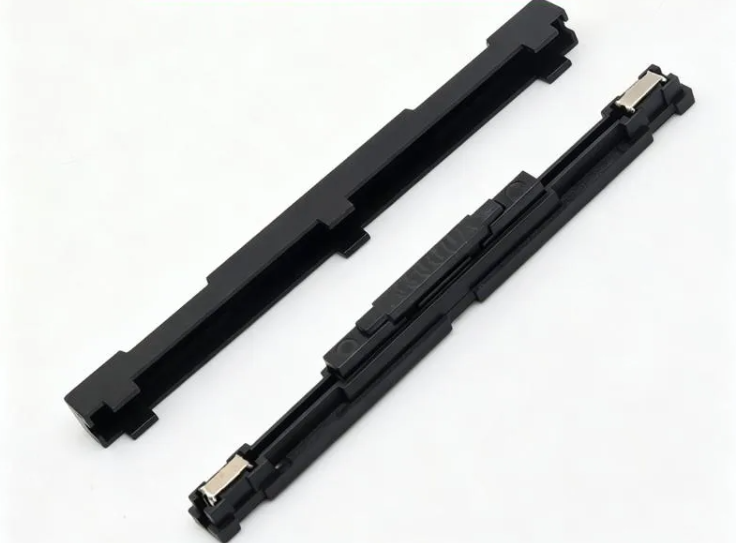
\includegraphics[width=\linewidth]{protector.png}}
    \caption{Proteccion para empalmes.}
    \label{fig:protector}
  \end{subfigure}
  \caption{Materiales Necesarios 2.}
  \label{fig:elementos2}
\end{figure}

\section{Procedimiento de Conexión de la Alimentación Externa}
\label{Anexo1}

\begin{itemize}
    \item \textbf{Fuente Externa:} Configurada en un rango de $9\,\text{V}$ a $15\,\text{V}$.
    \item \textbf{Conexión Positiva:} Borne positivo de la fuente a los bornes rojos 13 (Transmisor) y 19 (Receptor).
    \item \textbf{Conexión Negativa:} Borne negativo de la fuente a los bornes verdes 15 (Transmisor) y 21 (Receptor).
    \item \textbf{Control de Encendido:} Los interruptores de batería (2 en TX y 9 en RX) no tienen efecto con alimentación externa, por lo que el encendido/apagado se efectúa conectando/desconectando los cables de la fuente.
\end{itemize}
\newpage

\nocite{*}

\newpage
\printbibliography[heading=bibintoc, title={Bibliografía y Referencias}]
\end{document}
